\let\mymarginpar\marginpar

\documentclass[11pt]{article}


\usepackage{enumerate}% http://ctan.org/pkg/enumerate
\usepackage{amsmath} 
\usepackage{times}
\usepackage{amsmath,amsthm,amssymb}
\usepackage{fancyhdr}
\usepackage{moreverb}
\usepackage{graphicx}
\usepackage{amssymb}
\usepackage{url}
\usepackage{multirow} 
\usepackage[boxed]{algorithm}
%\usepackage[noend]{algpseudocode}
%\usepackage{algorithm}
%\usepackage{algorithmic}
\usepackage{algpseudocode}
%\usepackage{cite}
\usepackage{multirow,bigdelim}
\usepackage{geometry}
\usepackage{fix-cm}
%\usepackage{subfigure}
\usepackage{natbib}
\usepackage{color}
\usepackage{bbold}
\usepackage{graphicx}
\usepackage{caption}
\usepackage{subcaption}



\newcommand{\COR}{\text{COR}}
\newcommand{\POS}{\text{POS}}
\newcommand{\UNIT}{\text{UNIT}}
\newcommand{\LIN}{\text{LIN}}
\newcommand{\SD}{\text{SD}}

\newcommand{\myN}{\hbox{N\hspace*{-.9em}I\hspace*{.4em}}}
\newcommand{\myZ}{\hbox{Z}^+}
\newcommand{\myR}{\hbox{R}}
\newcommand{\R}{\mathbb{R}}
\newcommand{\PP}{{\bf P}}
\newcommand{\bLambda}{\boldsymbol{\lambda}}

\renewcommand{\P}{\mathbb{P}}
\newcommand{\E}{\mathbb{E}}
\newtheorem{defi}{Definition}
\newtheorem{theorem}{Theorem}[section]
\newtheorem{lemma}[theorem]{Observation}
\newtheorem{proposition}[theorem]{Proposition}
%\newtheorem{theorem}[theorem]{Theorem}
\newtheorem{observation}[theorem]{Observation}
\DeclareMathOperator*{\argmax}{arg\,max}
\DeclareMathOperator*{\argmin}{arg\,min}

\theoremstyle{definition}
\newtheorem{example}[theorem]{Example}

\theoremstyle{definition}
\newtheorem{definition}[theorem]{Definition}

\renewcommand{\abstractname}{}
\def\pb{\overline{p}}
\def\pt{\tilde{p}}
\def\one{{\bf 1}}

\def\bSigma{{\bf \Sigma}}
\def\bLambda{{\bf \Lambda}}
\def\blambda{\boldsymbol{\lambda}}
\def\bOmega{{\bf \Omega}}

\def\dd{{\bf d}}
\def\D{{\bf D}}
\def\v{{\bf v}}
\def\V{{\bf V}}
\def\s{{\bf s}}
\def\m{{\bf m}}
\def\r{{\bf r}}
\def\a{{\bf a}}
\def\x{{\bf x}}
\def\q{{\bf q}}
\def\w{{\bf w}}
\def\A{{\bf A}}
\def\M{{\bf M}}
\def\X{{\bf X}}
\def\Y{{\bf Y}}
\def\Q{{\bf Q}}
\def\L{{\bf L}}
\def\Beta{\boldsymbol{\beta}}
%\def\R{{\bf R}}
\def\Z{{\bf Z}}
\def\B{{\bf B}}
\def\SS{{\bf S}}
\def\I{{\bf I}}
\def\F{{\cal F}}
\def\G{{\cal G}}
%\def\L{{\cal L}}
\def\P{{\mathbb P}}
\def\E{{\mathbb E}}
\def\Var{{\rm Var}\,}
\def\Cov{{\rm Cov}\,}
\def\Corr{{\rm Corr}\,}
\def\ee{\varepsilon}
\def\|{\, | \,}
\def\probit{p_{\rm probit}}
\def\plog{p_{\rm log}}
\def\conv{\text{conv}}
\def\cond{\text{cond}}
\def\diag{\text{diag}}
\def\vech{\text{vech}}
\def\vec{\text{vec}}
\def\Diag{\text{Diag}}
\def\diag{\text{diag}}
\def\Tr{\text{tr}}

\def\logit{{\rm logit}}

\newcommand{\myzrfunction}[1]
{\myfunction{#1}{{\myZ}}{{\myR}}}

\allowdisplaybreaks
\newcommand{\mysection}[1]
{\noindent {\bf {#1}}}

\title{Combining and Extremizing Real-Valued Forecasts}

\author{
Ville A. Satop\"a\"a and Lyle H. Ungar} 
\date{}
%%%%%% Begin document with header and title %%%%%%%%%

\begin{document}
\maketitle

\begin{abstract}


\end{abstract}


\section{Introduction} \label{introduction}

Policy-makers often consult human or/and machine agents for forecasts
of some future outcome. For instance, multiple economics experts may
provide quarterly predictions of gross domestic product (GDP). Typically it is not possible to determine ex-ante which expert will be the most accurate, and even if this could be done, heeding only the most accurate expert's advice would ignore a potentially large amount of relevant information that is being contributed by the rest of the experts. Therefore a better alternative is to combine the
forecasts into a single consensus forecast that represents all the experts' advice. 
% is done both for
%the sake of decision-making and
%accuracy \citep{armstrong2}. 
The policy-makers, however, can choose to aggregate the forecasts in many different ways. The final choice of the combination rule is crucial because it often
significantly affects the predictive accuracy of the consensus
forecast. 



Possibly because of its simplicity and intuitive appeal, the most
popular approach to combining forecasts is the weighted average, sometimes also known as the linear opinion pool. 
This technique has a long tradition, with many empirical studies attesting to its benefits (see, e.g., \citealt{bates1969combination, clemen1989combining, armstrong2}). 
%For instance, 
%and has benefited a diverse range of fields such as meteorology \citep{sanders1963subjective, baars2005performance}, economics \citep{}
Even though the average forecast does not always outperform the best single forecaster \citep{hibon2005combine},
forecast averaging is still considered state-of-the-art \citep{elliott2013handbook}. Theoretically,  approximating the optimal weighted average under different forecasting setups and loss functions has been well-studied (see, e.g., \citealt{juditsky2008learning, degroot1991optimal}). Empirically, weighted averaging has become a well-established practice in economics \citep{blix2001good},  weather forecasting \citep{raftery2005using}, political science \citep{graefea2014combining}, and many other disciplines.
%
% organizations, including central banks, government institutions, and private companies.


\cite{Ranjan08} analyze the weighted average of probability forecasts of binary events, such as rain or no
rain tomorrow. They explain how the quality of a probability forecast
(individual or aggregate) is typically measured in terms of
\textit{reliability} and \textit{resolution} (sometimes also known as calibration and
sharpness, respectively). Reliability describes how closely the
conditional event frequencies align with the forecast
probabilities. Resolution, on the other hand, measures how far the
forecasts are from the naive baseline forecast, that is, the marginal
event frequency. A forecast that is reliable and highly resolute is
very useful to the policy-maker because it is both accurate and close
to the most confident values of zero and one. Therefore a
well-established goal in probability forecasting is to maximize resolution subject to
reliability \citep{murphy1987general, gneiting2007probabilistic}.


Strikingly, \cite{Ranjan08} prove that any non-trivial weighted average
of two or more different, reliable probability forecasts is
unreliable and lacks resolution. In particular, they explain that such
a weighted average is overly
close to the marginal event frequency and hence can be considered under-confident.  This result is an important
contribution to the probability forecasting literature in part
because it points out a dramatic shortcoming of methodology that is
used widely in practice. However, the authors neither provide a
principled way of addressing this shortcoming nor interpret potential causes of the under-confidence. 



%This paper presents a method of forecast
%aggregation that aims to combine information from multiple forecasts
%into a single forecast with optimal properties.

The first step towards addressing these issues and improving the general practice of aggregation  is to understand what is meant by principled aggregation. This topic was discussed by \cite{satopaamodeling2, satopaamodeling} who propose the \textit{partial information 
framework} as a general platform for combining forecasts. They assume forecast heterogeneity to stem from information available to the forecasters and how they decide to use it. For instance, forecasters studying the same (or different) articles about the state of the economy may use distinct parts of the information and hence report different predictions of the next quarter's GDP. Overall, the framework makes the same assumptions as \cite{Ranjan08} but provides concrete models with optimal aggregators. 
%combining information from multiple forecasts into a single forecast with optimal properties.
%optimally combining forecasts. 
For instance, the authors describe a Gaussian partial information model under which optimal aggregation is based on the covariance matrix of the individual forecasts. They apply this model to different types of synthetic and real-world data, and illustrate how it improves upon averaging and other types of measures of central tendency. Therefore the partial information framework is both intuitively and empirically appealing.
% but tends empirically explains real world forecasting reasonably well. 
%
% These issues can be handled by the partial information 
%framework \citep{satopaamodeling2, satopaamodeling} that 
% based on the covariance between the forecasters.

This paper analyzes weighted averaging under the general partial information framework. Our first contribution extends the result
in \cite{Ranjan08} to the weighted average of any type of univariate
forecasts, including real-valued forecasts.
%, and provides an algorithm that optimally (under a reasonable model) combines real-valued forecasts. 
This result shows, for instance, that any non-trivial
weighted average of predictions about the next quarter's GDP
is both unreliable and under-confident. The discussion
provides general, yet intuitive, descriptions of well-known properties
such as reliability and resolution. Furthermore, the analysis reveals a new property
that is satisfied by all optimal aggregators, namely, that the variance of
the aggregator is
never less than the maximum variance among the individual
forecasts. Showing that a non-trivial weighted average cannot satisfy
this condition leads to a mathematically precise yet
easy-to-understand explanation of why weighted averages are
under-confident.  Furthermore, this reasoning suggests that
under-confidence is not unique to the class of weighted averages but
extends to many other measures of central tendency, such as the
median.
% Therefore developing an alternate class of aggregators is almost certainly called for.
% and extends, in a different form, to real-valued estimates.

Under-confidence of a simple aggregator can be often alleviated by systematically transforming it away from the naive baseline forecast, namely the marginal mean of the outcome. 
%non-informative prior probability of $1/2$
This technique, known as \textit{extremizing}, is increasingly used in the probability forecasting literature as a means of
improving the average forecast. For instance, \cite{Ranjan08} propose a beta transformation that extremizes the weighted average of
  the probability forecasts; \cite{satopaa} use a logistic regression model to extremize the average log-odds of the
  forecasts; many others, including \cite{baron2014two}, \cite{mellers2014psychological}, and \cite{shlomi2010subjective}, have also discussed extremization. 
%   propose yet another extremizing  transformation.
% {\cite{Ranjan08,satopaa,baron2014two}.\footnote{Unfortunately, many different
%  ad hoc transformations have been used. 
%  For instance, \cite{Ranjan08} propose a beta transformation that extremizes the weighted average of
%  the probability forecasts; \cite{satopaa} use a logistic regression model to extremize the average log-odds of the
%  forecasts; \cite{baron2014two} propose yet another extremizing  transformation.}
Conceptually, extremizing is a very simple idea that can be applied to any kind of forecasts.
% -- not just to probability forecasts. 
 This paper suggests that extremizing can improve an aggregator also when the forecasts are real-valued. 
%is not a technique restricted to probability forecasting but should be also practiced even when the forecasts are real-valued.
Our second contribution illustrates this with a convex optimization procedure that linearly extremizes the weighted average of real-valued forecasts. The technique is applied to simple examples involving both synthetic and real-world data. In both examples extremizing leads to a significant improvement in resolution and reliability. In particular, the resulting aggregate exhibits many properties of optimal aggregation.

%Our second contribution illustrates this both on synthetic and real-world data.
%, extremizes the weighted average of real-valued forecasts, and shows how this
%that transforming the weighted average of real-valued forecasts further away from the  naive baseline forecast, namely the marginal mean of the outcome
%{\bf what does extremizing mean in the real-valued setting?}:
%This 
%can improve both its
%resolution and reliability.
% even when the forecasts are not
%probabilities of binary outcomes. 
%Our second contribution illustrates
%this with simple examples involving both synthetic and real-world data
%with outcomes defined on the entire real line.


The rest of the paper is structured as follows. Section \ref{propertiesS} briefly
introduces the general partial information framework and discusses some properties of
the optimal aggregator within that framework. The class of weighted
averages is then analyzed in the light of these optimal
properties. Section \ref{extremization} describes the optimization technique for extremizing the weighted average of
real-valued forecasts. Section \ref{simulation} illustrates this
technique and our theoretical results over simulated
data. Section \ref{application} repeats the analysis over real-world data. The final section
concludes and discusses future research directions.

\section{Forecast and Aggregation Properties} \label{propertiesS}
\subsection{Optimal Aggregation}


Consider $N$ forecasters and suppose forecaster $j$ predicts $X_j$ for
some (integrable) quantity of interest $Y$.  The partial information
framework assumes that $Y$ and $X_j$, for $j = 1, \dots, N$, are
measurable random variables under some common probability space
$(\Omega, \F , \P)$ (see \citealt{satopaamodeling}). Overall, this is similar to the setting
considered, for instance,
in \cite{degroot1981assessing}, \cite{murphy1987general}, and more
recently in \cite{Ranjan08}. Akin to \cite{Ranjan08}, the forecasters
are assumed to be \textit{reliable}, that is, conditionally unbiased
such that $\E(Y | X_j) = X_j$ for all $j = 1, \dots, N$.  To interpret
this assumption, observe that the principal $\sigma$-field $\F$ holds
all possible information that can be known about $Y$. For each
reliable forecast $X_j$ there exists a $\sigma$-field, namely
$\sigma(X_j) = \F_j \subseteq \F$ such that $X_j
= \E(Y|\F_j)$. Conversely, suppose that $X_j = \E(Y|\F_j)$ for some
$\F_j \subseteq \F$, then
\begin{align*}
\E(Y | X_j) &= \E[\E(Y|X_j,\F_j)|X_j] = \E[\E(Y|\F_j)|X_j] = \E(X_j|X_j) = X_j.
\end{align*}
Therefore a forecast is reliable if and only if it represents the optimal use of some information set, that is, it is consistent with some partial information $\F_j \subseteq \F$.
% it is consistent with some set of information about $Y$. In other words, $X_j$ represents the optimal use of some information set $\F_j \subseteq \F$.
%if there exists an information set $\F_j$ that, after being utilized optimally, leads to the forecast $X_j$, then $X_j$ is reliable (and \textit{vice versa}). 
 An aggregator is defined to be any forecast that is measurable with respect to $\F'' := \sigma(X_1, \dots, X_N)$, namely the $\sigma$-field generated by the individual forecasts. For the sake of notational clarity, aggregators are represented by different versions of the script symbol $\mathcal{X}$.



If $\E\left(Y^2\right) < \infty$, the conditional expectation
$\mathcal{X}'' := \E(Y | \F'')$ minimizes the expected quadratic loss
among all aggregators. This forecast is called the \textit{revealed
aggregator} because it optimally utilizes all the information that the
forecasters' reveal through their forecasts. Even though
$\mathcal{X}'' $ is typically too abstract to be applied in practice,
it provides an optimal baseline for aggregation
efficiency. Therefore studying its properties gives guidance for
improving aggregators currently used in practice. Some of these
properties are summarized in the following theorem. The proof of this
and any other theorems are deferred to the Appendix.



\begin{theorem} \label{optimal}
Suppose that $X_j = \E(Y | X_j)$ for all $j = 1, \dots, N$ and denote the revealed aggregator with $\mathcal{X}'' = \E(Y | \F'')$, where $\F'' = \sigma(X_1, \dots, X_N)$. 
%The individual forecasts agree with $Y$ in expectation, that is, $\E(X_j) = \E(Y) = \mu_0$. 
Let $\delta_{max} := \max_j \{ \Var(X_j)  \}$ be the maximal variance among the individual forecast.
% $\delta_{max} = \E[(\mu_0 - X_j)^2]$. 
 Then the following holds.
\begin{enumerate}[i)] \label{properties}
\item \textbf{Marginal Consistency.} $\mathcal{X}''$ is marginally consistent:  $\E(\mathcal{X}'') = \E(Y) :=  \mu_0$.
\item \textbf{Reliability.} $\mathcal{X}''$ is reliable: $\E(Y|\mathcal{X}'') = \mathcal{X}''$. 
\item \textbf{Variance Expansion.} $\mathcal{X}''$ is expanding: $\delta_{max} \leq \Var(\mathcal{X}'') \leq \Var(Y)$. In words, the variance of $\mathcal{X}''$ is always at least as large as that of the most variable forecast. 
\end{enumerate}
\end{theorem}
Marginal consistency states that the forecast and the outcome agree in expectation. If $X_j$ is reliable, then $\E(X_j) = \E[\E(Y|X_j)] = \E(Y) = \mu_0$. Consequently, all reliable forecasts (individual or aggregate) are marginally consistent. The converse, however, is not true. For instance, Theorem \ref{contraction} shows that any non-trivial weighted average is marginally consistent but unreliable. This is an important observation because it provides a technique for proving lack of reliability via marginal inconsistency -- a task that is generally much easier than disproving reliability directly.


Theorem \ref{optimal} bounds the variance of $\mathcal{X}''$. The upper bound holds for all reliable forecasts. This follows directly from the fact that each reliable forecast can be associated with a sub-$\sigma$-field and the fact that conditional expectation is a contraction in $L^2$ \citep[Theorem 5.1.4.]{durrett2010probability}. The key component, however, is the lower bound.
To provide intuition, consider the least informative $\sigma$-field, namely the trivial $\sigma$-field $\F_0 := \{\emptyset, \Omega\}$. A forecast based on $\F_0$ is always equal the marginal mean $\mu_0$ and hence has zero variance. On the other hand, a forecast based on all the information, namely the principal $\sigma$-field $\F$, is always equal to $Y$ and has variance $\Var(Y)$. 
The intermediate cases can be understood by considering an increasing sequence of $\sigma$-fields $\F_0 \subseteq \F_1 \subseteq \dots \subseteq \F_M \subseteq \F$ and the corresponding forecasts $X_m = \E(Y|\F_m)$ for $m = 1, \dots, M$. According to \citet[Proposition 2.1]{satopaamodeling2}, the variances of these forecasts respect the same order as their information sets. In other words, $\Var(X_1) \leq \Var(X_2) \leq \dots \leq \Var(X_M) \leq \Var(Y)$. This suggests that the amount of information used in a reliable forecast is quantified by variance. Naturally, if an aggregator pools information from forecasters, it should use at least as much information as the most informed individual forecaster.  In other words, its variance should exceed that of the individual forecasters'. Any reliable aggregator that satisfies this property is deemed (variance) \textit{expanding} and can be considered to collect information. 

Recall that in probability forecasting a well-established goal is to maximize resolution subject to reliability. This goal can be easily interpreted and understood in a more general context with the help of partial information. First, conditioning on reliability requires the forecast to be consistent with some set of information about $Y$. Maximizing the resolution of this forecast takes it as far from $\mu_0$ as possible. This is equivalent to increasing the variance of the forecast as close to the theoretical upper bound $\Var(Y)$ as possible. Therefore the goal is to maximize the amount of information that the forecast is consistent with. Intuitively, this is very reasonable and should be considered as the general goal in forecasting.



\subsection{Weighted Averaging} \label{contraction}

The rest of the paper analyzes the most commonly used aggregator, namely the weighted average. The following theorem shows that a non-trivial weighted average is neither expanding nor reliable and therefore can be considered suboptimal. A similar theorem does not hold for all linear combinations of the individual forecasts. For instance, Section \ref{simulation} describes a model under which the optimal aggregator $\mathcal{X}''$ is always a linear combination of the individual $X_j$'s.




\begin{theorem}\label{contraction}
Suppose that $X_j = \E(Y | X_j)$ for $j = 1, \dots, N$. Denote the weighted average with $\mathcal{X}_w = \sum_{j=1}^N w_jX_j$, where  $w_j \geq 0$ and $\sum_j w_j = 1$.  Let $j = \argmax_i \{ \Var(X_i)  \}$ identify the forecast with the maximal variance $\delta_{max} = Var(X_j)$. Then the following holds.
\begin{enumerate}[i)]
\item  $\mathcal{X}_w$ is marginally consistent.
\item $\mathcal{X}_w$ is not reliable, that is, $\P\left(\E(Y | \mathcal{X}_w) \neq \mathcal{X}_w\right) > 0$ if there exists a forecast pair $i \neq j$ such that $\P(X_i \neq X_j) > 0$ and $w_i, w_j > 0$. In words, $\mathcal{X}_w$ is necessarily unreliable if it assigns positive weight to at least two different forecasts. 
 
 \item Under the conditions of item ii), $\mathcal{X}_w$ lacks resolution. More specifically, if $\mathcal{X}_w' :=  \E(Y| \mathcal{X}_w)$ is the reliable version of $\mathcal{X}_w$, then $\E(\mathcal{X}_w) = \E(\mathcal{X}_w') = \mu_0$ but $\Var(\mathcal{X}_w) < \Var(\mathcal{X}_w')$. In other words, $\mathcal{X}_w$ is closer to the marginal mean $\mu_0$ than its reliable version $\mathcal{X}_w'$. \label{underconfA}
 
\item $\mathcal{X}_w$ is not expanding, that is, $\Var(\mathcal{X}_w) \leq \delta_{max}$. Therefore $\mathcal{X}_w$ is under-confident in a sense that it is as close or closer to the marginal mean $\mu_0$ than the revealed aggregator $\mathcal{X}''$.  Furthermore, $\Var(\mathcal{X}_w) = \Var(\mathcal{X}'')$ if and only if both $\mathcal{X}_w = \mathcal{X}'' = X_j$; that is,  $X_j$ provides all the information necessary for $\mathcal{X}''$, and the weighted average assigns all weight to $X_j$ (or to a group of forecasts all equal to $X_j$). \label{underconfB}
\end{enumerate}
\end{theorem}

Both items \ref{underconfA}) and \ref{underconfB}) discuss under-confidence but in a slightly different manner. Item \ref{underconfA}) is a direct generalization of the result in \cite{Ranjan08}. Intuitively, it states that if $\mathcal{X}_w$ is trained to use its information accurately, the resulting aggregator is more confident. Therefore under-confidence is defined with respect to the improved version of  $\mathcal{X}_w$. Under this kind of comparison, however, a reliable forecast is never under-confident. For instance, 
the marginal mean $\mu_0$ is reliable and hence would not be considered under-confident. Intuitively, however, it is clear that no forecast is more under-confident than $\mu_0$. To address this drawback, item \ref{underconfB}) measures under-confidence with respect to the optimal aggregator, namely the revealed aggregator instead. This comparison estimates whether the weighted average is as confident as it should be given the information it received through the forecasts. Item \ref{underconfB}) shows that this happens only if all the weight is assigned to a forecaster whose information set contains all the other forecasters' information. However, even if $\mathcal{X}_w$ could pick out the most informed forecaster ex-ante, the chances of this forecaster knowing everything that the rest of the forecasters know is extremely small in practice. In essentially all other cases, $\mathcal{X}_w$ is unreliable 
and hence not consistent with some set of information about $Y$. Consequently, its variance cannot be interpreted as the amount of used information. 

In general, many measures of central tendency reduce variance and hence are also separated from the revealed aggregator by the maximum variance among the forecasts. For instance, \cite{papadatos1995maximum} discuss the maximum variance of different order statistics and show that the variance of the median is upper bounded by the global variance of the individual forecasts. Such measures are not expanding and cannot be considered to aggregate information. In fact, \cite{satopaamodeling} explain that averaging-like techniques work well when the individual forecasters have very similar sets of information, that is, when there really is no information aggregation problem to begin with. Averaging-like aggregators are designed to reduce ``measurement error,'' which is philosophically very different to the idea of information aggregation discussed in this paper. In particular, under measurement error an aggregator with a relatively high variance is generally considered to be less precise. This stands in sharp contrast with what increased variance represents under partial information. 


Given that averaging aggregators are under-confident, a simple adjustment is to  increase their variance by transforming them systematically away from the marginal mean $\mu_0$. This is precisely what extremizing does. Therefore it is not surprising that extremizing has been observed to improve the predictive accuracy of many simple aggregators of  probability forecasts. To the best of our knowledge, however,  no previous study has illustrated the benefits of extremizing real-valued forecasts. This is the main focus in the remainder of the paper.

%The next section introduces a simple optimization procedure that extremizes the weighted average of real-valued forecasts. 


\section{Extremizing Real-Valued Forecasts} \label{extremization}

Estimating the weights and the amount of extremization requires the forecasters to address more than one related problems. For instance, they may participate in separate yet similar prediction problems or give repeated forecasts on a single recurring event. Across such problems the weights and the resulting under-confidence are likely to remain stable, allowing the aggregator parameters to be estimated based on multiple predictions per forecaster. For these reasons, suppose that the forecasters address $K \geq 2$ problems. Denote the outcome of the $k$th problem with $Y_k \in \mathbb{R}$ and let $X_{jk} \in \mathbb{R}$ represent the $j$th forecaster's prediction for this outcome. Assume that these variables are centered around a common marginal mean $\mu_0$.  



Extremization requires at least two parameters: the prior mean, which acts as the pivot point and decides the direction of extremizing, and the amount of extremization itself.  In general, extremization is a very simple idea and could be performed in many different ways. However, if $\mathcal{X}_k^*$ denotes the extremized version of the weighted average for the $k$th problem, then probably the simplest and most natural formulation is the following:
\begin{align*}
\mathcal{X}_k^* = \alpha  \left(  \w'\X_{k} - \mu_0\right) + \mu_0,
\end{align*}
 where $\X_k = (X_{1k}, \dots, X_{Nk})'$, $\w = (w_1, \dots, w_N)'$ is the weight vector, and $\alpha \in (1, \infty)$ (or $\alpha \in [0, 1)$) leads to extremization (or contraction, respectively). If $\alpha = 1$, then $\mathcal{X}^*$ is equal to the weighted average $\mathcal{X}_w$.  This linear form is particularly convenient because it maintains the marginal consistency property of $\mathcal{X}_w$; that is, $\E(\mathcal{X}^*) = \mu_0$ for all values of $\alpha$.  However, $\Var(\mathcal{X}^*)$ increases in $\alpha$ such that $\Var(\mathcal{X}^*) = \alpha^2 \Var(\mathcal{X}_w) > \Var(\mathcal{X}_w)$ for all $\alpha > 1$. Therefore, for a large enough $\alpha$, $\mathcal{X}^*$ is both marginally consistent and expanding. These properties hold even if the weighted average is replaced by some other marginally consistent aggregator. However, given that the main purpose of this procedure is to illustrate Theorem \ref{contraction}, only the weighted average is considered for extremization.

Recall that the forecasts are marginally consistent with the outcomes. Therefore an unbiased estimator of the prior mean $\mu_0$ is given by the sample average $\frac{1}{NK} \sum_{k=1}^K\sum_{j=1}^N X_{jk}$ or, alternatively, by $\frac{1}{K} \sum_{k=1}^K Y_k$. Estimating $\mu_0$ in this manner, however, leads to a two-step estimation procedure. A more direct approach is to estimate all the aggregator parameters, namely $\alpha$, $\mu_0$, and $\w$, jointly over some criterion. If $Y_k$ has an explicit likelihood in terms of $\mathcal{X}^*$, then the parameter values can be estimated by maximizing this likelihood. Assuming an explicit parametric form, however, can be avoided by recalling from Section \ref{contraction} that the revealed aggregator $\mathcal{X}''$ utilizes the forecasters' information optimally and minimizes the expected quadratic loss among all functions measurable with respect to $\F''$. Ideally, $\mathcal{X}^*$ would behave similarly to $\mathcal{X}''$. Therefore it makes sense to estimate its parameters by minimizing the average quadratic loss over the $K$ problems. Section \ref{simulation} shows that this is likely to improve both the resolution and reliability of the weighted average. 

These considerations lead to the following estimation problem:
\begin{align}
 \label{firstProblem}
 \begin{split}
\text{minimize } & \sum_{k=1}^K \left[ \alpha  \left(  \w'\X_{k} - \mu_0\right) + \mu_0 - Y_k \right]^2\\
\text{subject to } & w_j \geq 0 \text{ for } j = 1, \dots, N\\
& \sum_{j=1}^N w_j = 1\\
& \alpha \geq 0.
\end{split}
\end{align}
To express this problem in a form that is more amenable to estimation, denote an $N \times N$ identity matrix with $\I_N$,  a vector of $K$ ones with $\one_K$, and a vector of $N$ zeros with $\boldsymbol{0}_N$. If $\Y = (Y_1, \dots, Y_K)'$, $\X = (\one_K, (\X_1, \dots, \X_K)')$, and $\A = (\boldsymbol{0}_N, \I_N)$, then  problem (\ref{firstProblem}) is equivalent to
\begin{align}
 \label{secondProblem}
 \begin{split}
\text{minimize } & \frac{1}{2} \Beta' \X'\X \Beta - \Y'\X\Beta\\
\text{subject to } & -\A\Beta \leq \boldsymbol{0}_N,
\end{split}
\end{align}
where the inequality is interpreted element-wise and $\Beta$ is a vector of $N+1$ optimization parameters. Given that $\X'\X$ is always positive semidefinite, problem (\ref{secondProblem}) is a convex quadratic program that can be solved efficiently with standard optimization techniques. 
%For instance, our implementation uses a commercial optimization solver, called Gurobi \citep{gurobi}
 
 If $\Beta^* = (\beta_0^*, \dots, \beta_{N}^*)'$ represents the solution, the optimal values of the original parameters are recovered by
\begin{align*}
\alpha^* &= \sum_{j=1}^N \beta_j^*,\\
w_j^* &=  \beta_j^*/\alpha^* \text{ for } j = 1, \dots, N, \text{ and}\\
\mu_0^* &= -\beta_0^*/(1-\alpha^*).
\end{align*}
Observe that the solution to (\ref{secondProblem}) is nothing more than the ordinary least squares estimates under non-negativity constraints on the slope coefficients. Therefore a possible relaxation is to ignore these constraints and simply fit a multiple linear regression model with $\Y$ as response and $\X$ as the predictor. For the sake of correctness, however, this paper does not consider this relaxation but performs extremization via (\ref{secondProblem}). 

\section{Simulation Study} \label{simulation}

This section illustrates Theorem \ref{contraction} on data generated from the Gaussian partial information model introduced in \cite{satopaamodeling2, satopaamodeling} as a particularly close specification of the general partial information framework. They apply the Gaussian model to different real-world applications and show that it leads to accurate aggregation of both real-valued and probability forecasts. This suggests that the model is, at least to some degree, a reasonable approximation of real-world forecasting. 

The simplest version of this model occurs when the outcome $Y$ and the forecasts $X_j$ are real-valued with mean zero. The observables are then generated jointly from the following multivariate Gaussian distribution:
\begin{align}
\left(\begin{matrix} Y \\ X_{1}\\ \vdots \\ X_{N} \end{matrix}\right) &\sim \mathcal{N}_{N+1}\left( 
 \boldsymbol{0}, \left(\begin{matrix} 
1 & \diag(\bSigma)'\\
\diag(\bSigma) &\bSigma\\
 \end{matrix}\right) 
 :=
 \left(\begin{array}{c | c c cc }
1 & \delta_1 & \delta_2 & \dots & \delta_N  \\ \hline
\delta_1 & \delta_1 &\rho_{1,2} & \dots & \rho_{1,N}   \\ 
\delta_2 & \rho_{2,1} & \delta_2 & \dots & \rho_{2,N}  \\ 
\vdots & \vdots & \vdots & \ddots & \vdots  \\ 
\delta_N & \rho_{N,1} & \rho_{N,2} & \dots & \delta_N\\ 
 \end{array}\right)\right),  \label{NExperts}
\end{align}
where the covariance structure describes the information among the forecasters. In particular, the maximum amount of information is $1.0$. The diagonal entry $\delta_j \in [0,1]$ represents the amount of information known to forecaster $j$. A forecaster with $\delta_j = 1$ (or $\delta_j = 0$) always reports the correct answer $Y$ (or the marginal mean $\mu_0 = 0$, respectively). The off-diagonal $\rho_{i,j}$, on the other hand, can be regarded as the amount of information overlap between forecasters $i$ and $j$. Based on the well-known conditional distributions of a multivariate Gaussian (see, e.g., \citealt{ravishanker2001first}), the distribution of $Y$ conditional on forecast $X_j$ is $Y|X_j \sim \mathcal{N}(X_j, 1-\delta_j)$. This directly gives $\E(Y | X_j) = X_j$. Therefore the forecasts $X_j$ are reliable.
%shows that the forecast $X_j$ is reliable, that is, $\E(Y | X_j) = X_j$. 
According to the same conditional results, the distribution of $Y_k$ given all the forecasts, namely $\X_k$ is $Y_k | \X_k \sim \mathcal{N}(\diag(\bSigma)'\bSigma^{-1}\X_k, 1- \diag(\bSigma)'\bSigma^{-1}\diag(\bSigma))$. This in turn shows that the revealed aggregator for the $k$th problem is  $\mathcal{X}_k''  = \E(Y_k | \X_k) = \diag(\bSigma)'\bSigma^{-1}\X_k$. 

%This aggregator represents optimal use of the forecasters' revealed information. 

%\marginpar{This aggregator extremizes; it never reduces to a weighted average as was shown in Proposition of satioaamodeling2}


\begin{figure}[t!]
        \centering
        \begin{subfigure}[b]{0.49\textwidth}
                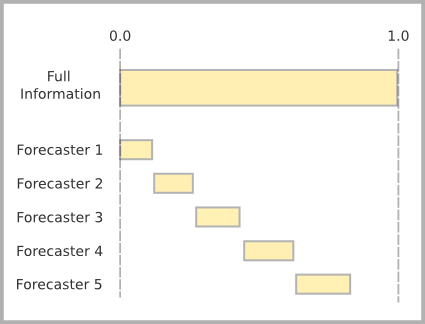
\includegraphics[width=\textwidth]{IndepDiagram}
                \caption{No Information Overlap}
                \label{DiagramsA}
        \end{subfigure}%
        ~ %add desired spacing between images, e. g. ~, \quad, \qquad, \hfill etc.
          %(or a blank line to force the subfigure onto a new line)
        \begin{subfigure}[b]{0.49\textwidth}
                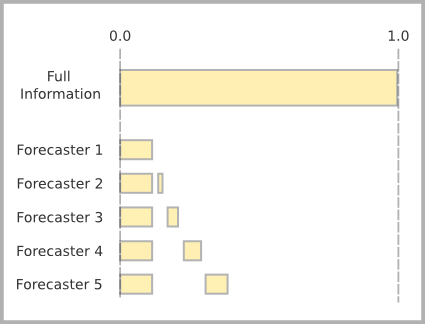
\includegraphics[width=\textwidth]{DepDiagram}
                \caption{High Information Overlap}
                \label{DiagramsB}
        \end{subfigure}
   \caption{Diagram illustration of the information distribution among $N = 5$ forecasters. The top bar next to \textit{Full Information} represents all possible information that can be known about $Y$. The bars leveled horizontally with \textit{Forecaster $j$}, on the other hand, represent the information used by that forecaster.}    
        \label{Diagrams}
\end{figure}


The simulation study considers $N = 5$ forecasters under two different information scenarios: 
\begin{enumerate}
\item[] \textit{No Information Overlap.}  Fix $\delta_j = 0.1 + 0.02j$ for $j = 1, \dots, 5$ and let $\rho_{i,j} = 0$ for all $i,j$. Therefore the forecasters have independent information sources. This scenario is illustrated in Figure \ref{DiagramsA}. Summing up the individual variances shows that as a group the forecasters know $80\%$ of the total information. The revealed aggregator simplifies to $\mathcal{X}_k'' = \sum_{j=1}^5 X_{jk}$, has variance $0.80$, and therefore uses all available information.


\item[] \textit{High Information Overlap.} Fix $\delta_j = 0.1 + 0.02j$ for $j = 1, \dots, 5$ and let $\rho_{i,j} = 0.12$ for all $i,j$. Therefore the forecasters have significant information overlap and as a group know only $32\%$ of the total information. This scenario is illustrated in Figure \ref{DiagramsB}. The revealed aggregator simplifies to $ \mathcal{X}_k'' = \left( \sum_{j=2}^5 X_{jk} \right) - 3X_{1k}$, has variance $0.32$, and therefore uses all available information.
\end{enumerate}


The competing aggregators are the equally weighted average $\bar{\mathcal{X}}$, the optimally weighted average $\mathcal{X}_w$, and the extremized version of the optimally weighted average $\mathcal{X}^*$. The parameters in $\mathcal{X}^*$ and  $\mathcal{X}_w$ are first estimated by minimizing the average quadratic loss over a training set of $10,000$ draws from (\ref{NExperts}).  After this, all the competing aggregators are evaluated on an independent test set of $10,000$ draws from (\ref{NExperts}). 
%Finally,  the aggregators' performance is evaluated solely based on out-of-sample accuracy.
Therefore all the following results, apart from the parameter estimates, represent out-of-sample performance. 



In probability forecasting the quality of the predictions is typically assessed using a reliability diagram. The idea is to first sort the outcome-forecast pairs into some number of bins based on the forecasts and then plot the average forecast against the average outcome within each bin. Figures \ref{NOVerlap} and  \ref{HighOverlap}  generalize this to continuous outcomes by replacing the conditional empirical event frequency with the conditional average outcome. Each bin is chosen to contain the same number of forecast-outcome pairs. The vertical dashed line represents the marginal mean $\mu_0 = 0$.  The plots have been scaled such that the identity function shows as the diagonal. Any deviation from this diagonal suggests lack of reliability. The grey area represents the reliability diagrams of a $1,000$ bootstrap samples of the forecast-outcome pairs. Therefore it serves as a visual guide for assessing uncertainty. The inset histograms help to assess resolution by comparing the empirical distribution of the forecasts against the prior distribution of $Y$, namely the standard Gaussian distribution represented by the red curve. In particular, if the forecast is reliable, then the closer its empirical distribution is to the standard Gaussian, the more information is being used in the forecast. 

% latex table generated in R 3.2.0 by xtable 1.7-4 package
% Wed May 20 21:31:51 2015
\begin{table}[ht]
\centering
\caption{The estimated parameter values 
%optimally weighted average, $\mathcal{X}_w$ and the extremized version of the optimally weighted average, $\mathcal{X}^*$
 under simulated data. }
\begin{tabular}{llrrrrrrr}
  \hline \hline
Scenario & Forecast & $\mu_0$ & $\alpha$ & $w_1$ & $w_2$& $w_3$& $w_4$& $w_5$ \\ 
  \hline
\multirow{2}{*}{No Overlap} & $\mathcal{X}_w$ &  &  & 0.0000 & 0.1080 & 0.2293 & 0.3025 & 0.3601 \\ 
&   $\mathcal{X}^*$ & 0.0004 & 5.0137 & 0.1964 & 0.2023 & 0.2008 & 0.2006 & 0.2000 \\ \rule{0pt}{2.9ex} 
\multirow{2}{*}{High Overlap}  & $\mathcal{X}_w$ &  &  & 0.0000 & 0.0000 & 0.0440 & 0.4262 & 0.5298 \\ 
  & $\mathcal{X}^*$ & -0.0077 & 1.3048 & 0.0000 & 0.0000 & 0.1456 & 0.3959 & 0.4585 \\ 
   \hline
\end{tabular}
\label{NoParams}
\end{table}


\begin{figure}[t!]
        \centering
        \begin{subfigure}[b]{0.323\textwidth}
                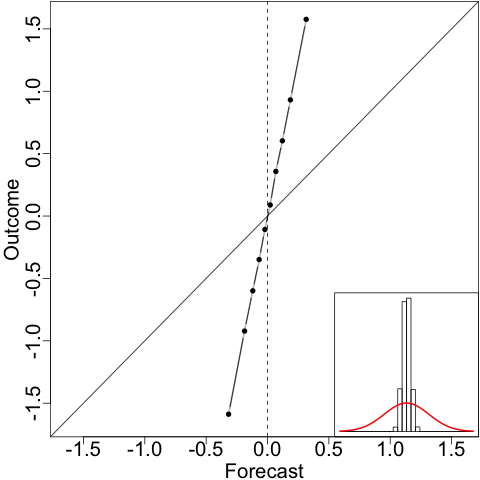
\includegraphics[width=\textwidth]{SimIndepELP}
                \caption{$\bar{\mathcal{X}}$}
        \label{RelEWANo}
        \end{subfigure}%
        ~ %add desired spacing between images, e. g. ~, \quad, \qquad, \hfill etc.
          %(or a blank line to force the subfigure onto a new line)
        \begin{subfigure}[b]{0.323\textwidth}
                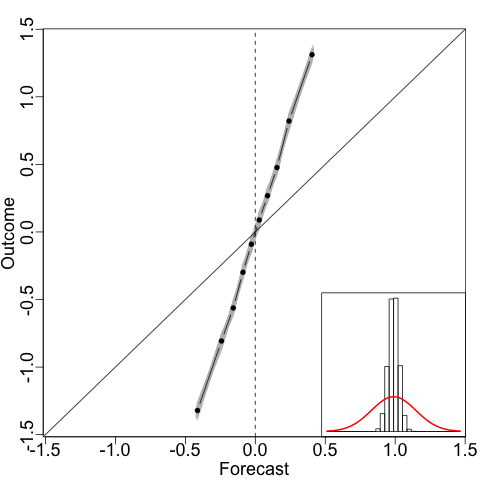
\includegraphics[width=\textwidth]{SimIndepOLP}
                \caption{$\mathcal{X}_w$}
        \label{RelOWANo}
        \end{subfigure}
        ~ %add desired spacing between images, e. g. ~, \quad, \qquad, \hfill etc.
          %(or a blank line to force the subfigure onto a new line)
        \begin{subfigure}[b]{0.323\textwidth}
                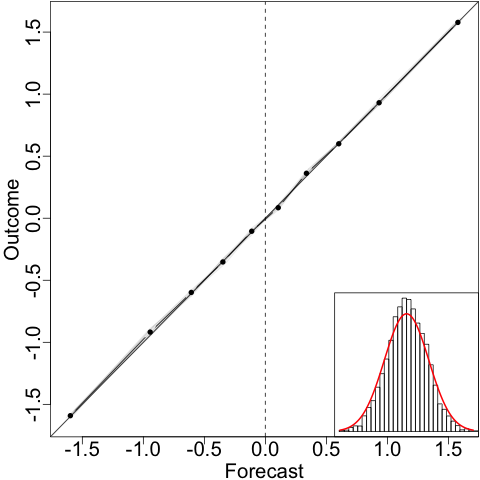
\includegraphics[width=\textwidth]{SimIndepELOP}
                \caption{$\mathcal{X}^*$ }
        \label{RelEOWANo}
        \end{subfigure}
   \caption{\textit{No Overlap.} Reliability diagrams of the competing aggregators  under simulated data. }
        \label{NOVerlap}
\end{figure}


\begin{figure}[t!]
        \centering
        \begin{subfigure}[b]{0.323\textwidth}
                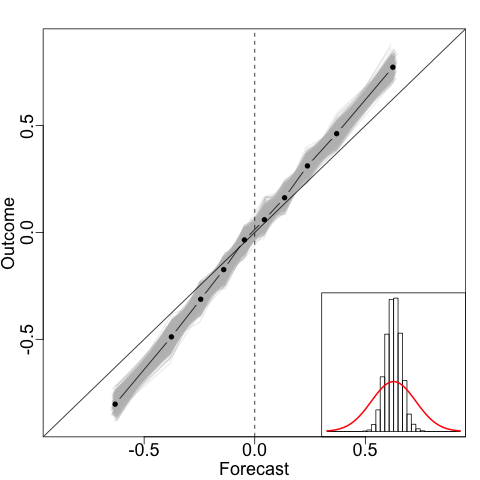
\includegraphics[width=\textwidth]{SimDepELP}
                \caption{$\bar{\mathcal{X}}$}
        \label{RelEWAHigh}
        \end{subfigure}%
        ~ %add desired spacing between images, e. g. ~, \quad, \qquad, \hfill etc.
          %(or a blank line to force the subfigure onto a new line)
        \begin{subfigure}[b]{0.323\textwidth}
                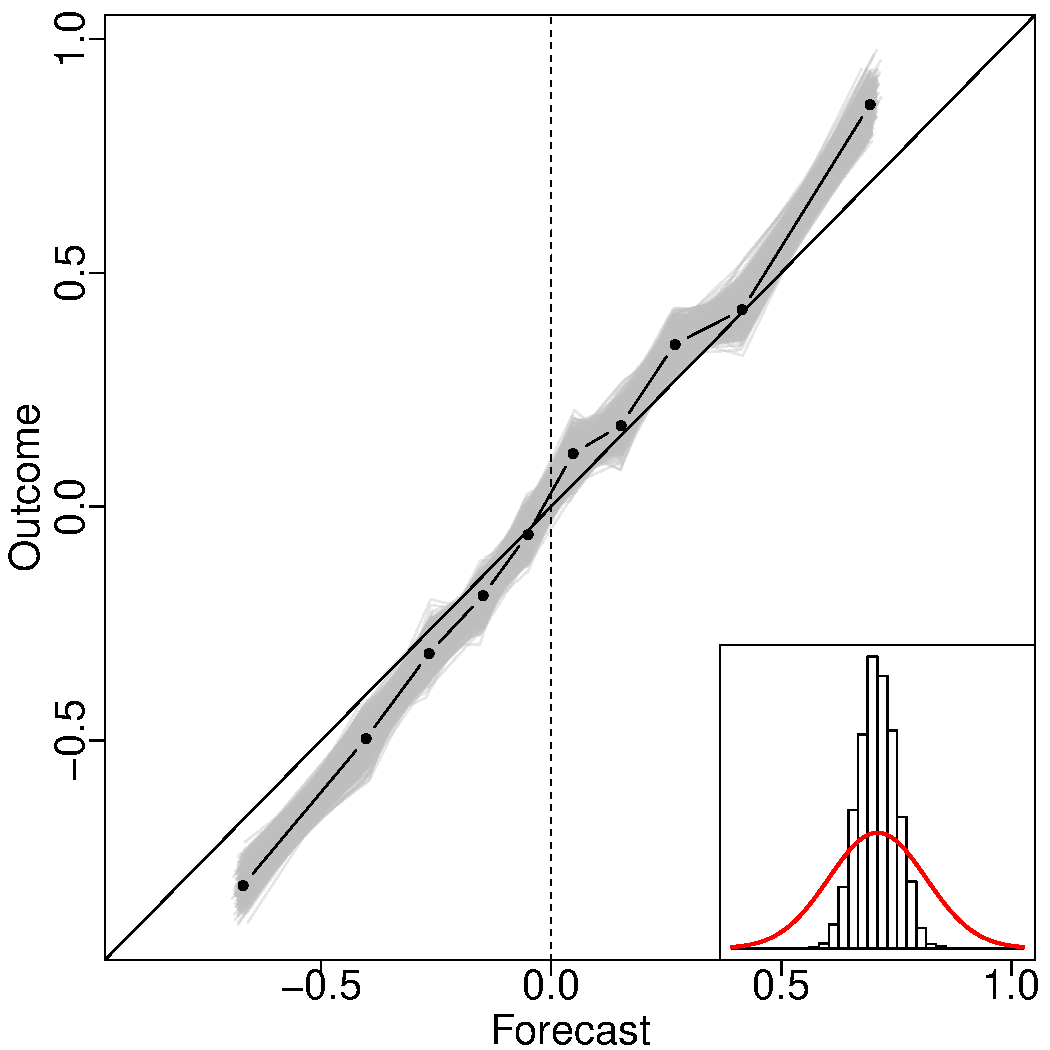
\includegraphics[width=\textwidth]{SimDepOLP}
                \caption{$\mathcal{X}_w$}
        \label{RelOWAHigh}
        \end{subfigure}
        ~ %add desired spacing between images, e. g. ~, \quad, \qquad, \hfill etc.
          %(or a blank line to force the subfigure onto a new line)
        \begin{subfigure}[b]{0.323\textwidth}
                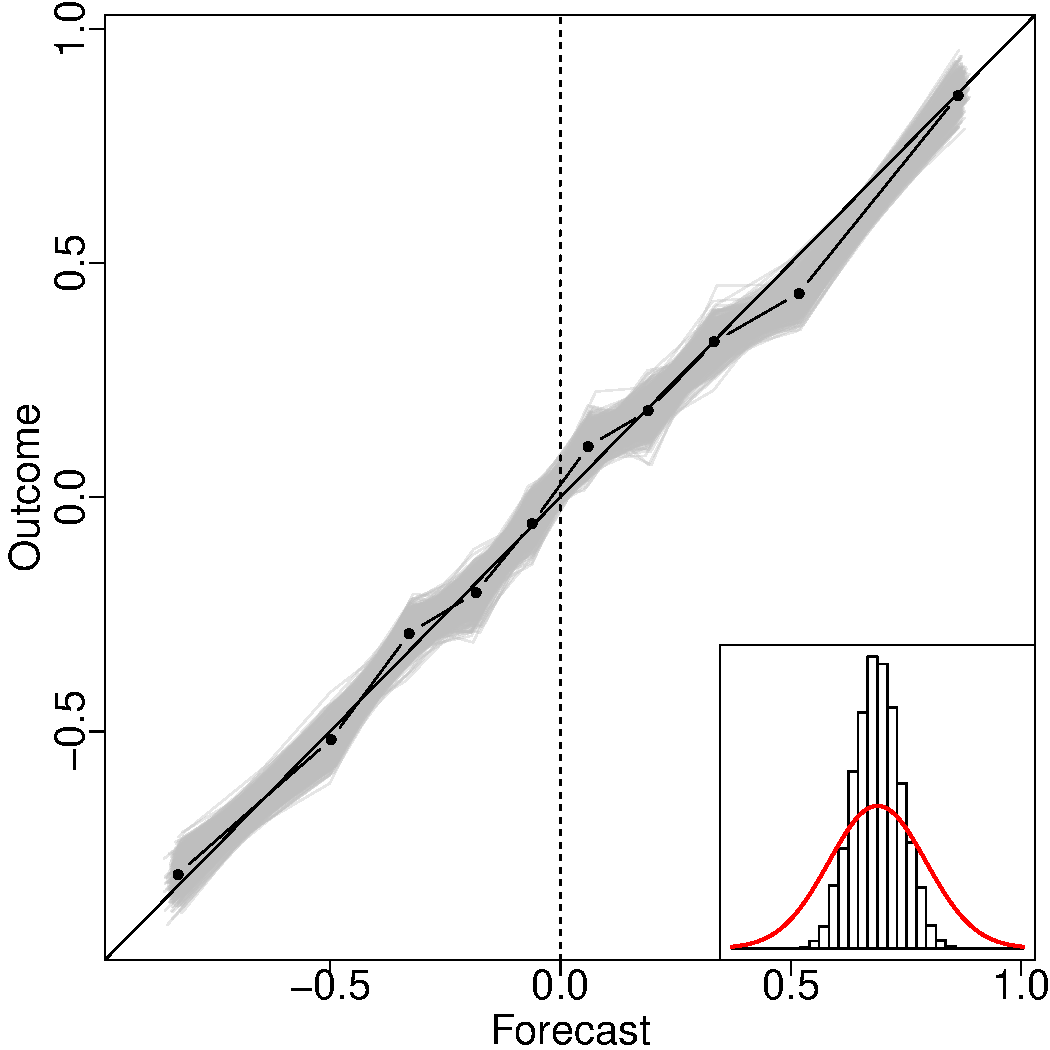
\includegraphics[width=\textwidth]{SimDepELOP}
                \caption{$\mathcal{X}^*$ }
        \label{RelEOWAHigh}
        \end{subfigure}
   \caption{\textit{High Overlap.} Reliability diagrams of the competing aggregators under simulated data. 
    }        
   \label{HighOverlap}
\end{figure}


According to Figures \ref{NOVerlap} and  \ref{HighOverlap}, the averaging aggregators, $\bar{\mathcal{X}}$ and $\mathcal{X}_w$ are unreliable and under-confident in both scenarios. The level of under-confidence is particularly startling in Figures \ref{RelEWANo} and \ref{RelOWANo} but decreases somewhat as overlap is introduced in Figures \ref{RelEWAHigh} and \ref{RelOWAHigh}. Given that averaging-like techniques do not behave like information aggregators, that is, they are not expanding, it is not surprising to see them perform better under high information overlap when aggregating information is less important for good performance. Table \ref{NoParams} shows the parameter estimates for $\mathcal{X}_w$ and $\mathcal{X}^*$.  The weights in $\mathcal{X}_w$ increase in the forecaster's amount of information, namely $\delta_j$ and differ noticeably from the equal weights employed by $\bar{\mathcal{X}}$. 
%The weights in $\mathcal{X}_w$ increase in the forecaster's amount of information, namely $\delta_j$ and differ noticeably from the equal weights employed by $\bar{\mathcal{X}}$. 
More importantly, however, in both information scenarios the extremizing parameter $\alpha > 1$. This reflects the need to correct the under-confidence of the traditional weighted average. The resulting $\mathcal{X}^*$ is more reliable and confident in both information scenarios.  In Figure \ref{RelEOWANo} its distribution appears to approximate the distribution of $Y$ very well, suggesting  almost complete information. Some of this information, however, is lost in Figure \ref{RelEOWAHigh} because in this scenario the group of forecasters knows $32\%$ of the total information, as opposed to the $80\%$ in the no overlap scenario.


%Table \ref{NoParams} shows the parameter estimates for $\mathcal{X}_w$ and $\mathcal{X}^*$. T



In addition to performing visual assessment, the aggregators can be compared based on their out-of-sample average quadratic loss. To make this specific, let $\Y = (Y_1, \dots, Y_K)$ collect all the outcomes of the testing problems and $\boldsymbol{\mathcal{X}} = (\mathcal{X}_1, \dots, \mathcal{X}_K)$ be a vector of some aggregate forecasts for the same problems. Then, the average quadratic loss for this aggregator is
\begin{align*}
L\left(\Y, \boldsymbol{\mathcal{X}}\right) &= \frac{1}{K} \sum_{k=1}^K \left(Y_k - \mathcal{X}_k\right)^2.
\end{align*}
If the forecasts are probabilities of binary outcomes, the above loss is called the Brier score and is known to have a decomposition that permits a closer analysis of  reliability and resolution. The decomposition, however, is not limited to probability forecasts. To see this, suppose that the real-valued aggregate $\mathcal{X}_k \in \{f_1, \dots, f_I\}$ for some finite number $I$. Let $K_i$ be the number of times $f_i$ occurs, $\bar{Y}_i$ be the empirical average of $\{Y_k : \mathcal{X}_k = f_i\}$, and $\bar{Y} = \frac{1}{K} \sum_{k=1}^K Y_k$. Then,
\begin{align}
L\left(\Y, \boldsymbol{\mathcal{X}} \right)  &= \underbrace{\frac{1}{K} \sum_{i=1}^I K_i(f_i - \bar{Y}_i)^2}_\text{REL} - \underbrace{\frac{1}{K} \sum_{i=1}^I K_i(\bar{Y}_i-\bar{Y})^2}_\text{RES} + \underbrace{\frac{1}{K} \sum_{k=1}^K (Y_k - \bar{Y})^2}_\text{UNC}. \label{decomposition}
\end{align}
See the Appendix for the derivation of this decomposition. Low REL suggests high reliability. If the aggregate is reliable, then RES is approximately equal to the sample variance of the aggregate and 
is positively associated with high resolution. 
%measures resolution; in particular, large RES indicates high resolution. 
The final term, UNC does not depend on the forecasts. This is the sample variance of $Y$ and therefore gives an approximate upper bound on the variance of any reliable forecast. As has been mentioned before, the goal is to maximize resolution subject to reliability. This decomposition shows how the quadratic loss addresses reliability and resolution simultaneously and therefore provides a convenient loss function for learning aggregation parameters. 


% latex table generated in R 3.1.2 by xtable 1.7-4 package
% Thu May  7 14:19:19 2015
\begin{table}[h!]
\centering
\caption{The average quadratic loss, $L(\Y,\boldsymbol{\mathcal{X}} )$ with its three additive components: reliability (REL), resolution (RES), and uncertainty (UNC). The final column, $s(\boldsymbol{\mathcal{X}} )$ gives the estimated variance of the forecast.} 
\begin{tabular}{llrrrrr}
  \hline \hline
Scenario & Forecast & $L(\Y,\boldsymbol{\mathcal{X}} )$ & REL & RES & UNC & $s(\boldsymbol{\mathcal{X}} )$ \\ 
  \hline
 \multirow{6}{*}{No Overlap} & Best Individual & 0.8024 & 0.0050 & 0.2108 & 1.0081 & 0.200\\ 
  & Median & 0.7322 & 0.2928 & 0.5688 & 1.0081& 0.046\\ 
  & $\bar{\mathcal{X}}$ & 0.7185 & 0.5140 & 0.8036 & 1.0081 & 0.032\\ 
  & $\mathcal{X}_w$ & 0.7016 & 0.2913 & 0.5979 & 1.0081 & 0.055\\ 
  & $\mathcal{X}^*$  & 0.1971 & 0.0022 & 0.8132 & 1.0081& 0.799\\ 
  & $\mathcal{X}''$ & 0.1969 & 0.0021 & 0.8132 & 1.0081 & 0.807\\ \rule{0pt}{2.9ex} 
  \multirow{6}{*}{High Overlap} &  Best Individual & 0.8141 & 0.0061 & 0.2195 & 1.0275 &0.199\\ 
  & Median & 0.8492 & 0.0087 & 0.1870 & 1.0275 &0.125 \\ 
  & $\bar{\mathcal{X}}$ & 0.8254 & 0.0137 & 0.2157 & 1.0275 &0.128\\ 
  & $\mathcal{X}_w$ & 0.7889 & 0.0166 & 0.2552 & 1.0275 &0.150 \\ 
  & $\mathcal{X}^*$  & 0.7758 & 0.0056 & 0.2573 & 1.0275 &0.228 \\ 
  &$\mathcal{X}''$ & 0.6837 & 0.0057 & 0.3496 & 1.0275 &0.318 \\ 
   \hline
\end{tabular}
\label{scenA}
\end{table}

Table \ref{scenA} presents the quadratic loss, its additive components, and the estimated variance $s(\boldsymbol{\mathcal{X}} )$ for each of the different forecasts under both information scenarios. In addition to the aforementioned $\bar{\mathcal{X}}$, $\mathcal{X}_w$, and $\mathcal{X}^*$, the tables also present scores for the median forecast,  the individual forecaster with the lowest quadratic loss, and the revealed aggregator $\mathcal{X}''$. According to the results, the best individual forecaster is reliable but extremely non-resolute, leading to an overall poor average quadratic loss. Under no information overlap, the best individual is better than both the median and $\bar{\mathcal{X}}$ because these aggregators assign too much importance to the individual forecasters with very little information. The median is the aggregator with the overall worst performance.  As predicted by Theorem \ref{contraction},  the averaging aggregators $\bar{\mathcal{X}}$ and $\mathcal{X}_w$ are neither reliable nor expanding. 

 The remaining two aggregators, namely $\mathcal{X}^*$ and $\mathcal{X}''$, on the other hand, are reliable, expanding, and resolute. Table \ref{NoParams} shows that $\mathcal{X}^*$ is in fact  almost equivalent to $\mathcal{X}''$ under no information overlap. Under high information overlap, however, $\mathcal{X}''$ gains slight advantage over $\mathcal{X}^*$. In this case $\mathcal{X}^*$ cannot take the same form as $\mathcal{X}''$. Consequently, it has a sample variance of $0.228$ which is well below the  amount of information known to the group, namely $0.320$. It fails to use information optimally because it cannot subtract off the shared information $X_1$ and hence avoid double-counting of information. However, despite it using information less efficiently, $\mathcal{X}^*$ is as reliable as $\mathcal{X}''$. Of course, under the Gaussian model it may be possible to compute $\mathcal{X}''$ directly. This, however, involves the non-trivial task of estimating the covariance matrix $\bSigma$ under a particular semidefinite constraint (see \citealt{satopaamodeling2} for more details). Solving the quadratic program (\ref{secondProblem}) is significantly easier. On the other hand, problem (\ref{secondProblem}) requires a training set with known outcomes whereas $\bSigma$ can be learned directly from the forecasts alone. Therefore the two aggregators can be seen to serve somewhat different purposes. 


\section{Case Study: Concrete Compressive Strength} \label{application}

Concrete is the most important material in civil engineering. One of its key properties is compressive strength that depends on the water-to-cement ratio but also on several other ingredients. \cite{yeh1998modeling} illustrated this by statistically predicting compressive strength based on age and seven mixture ingredients. The associated dataset is freely available at the UC Irvine Machine Learning Repository \citep{Lichman:2013} and consists of $1,030$ observations with the following information:

\begin{equation}
\begin{array}{ll r lr}
&&Y: & \text{Compressive Strength}&\\
\ldelim\{{8}{2.5em}[$\mathcal{M}_F$] &\ldelim\{{4}{2.5em}[$\mathcal{M}_1$] &V_1: &  \text{Cement (kg in a $m^3$ mixture)}&  \\
&&V_2: & \text{Coarse Aggregate (kg in a $m^3$ mixture)}&\\
  &&V_3: &  \text{Fly Ash (kg in a $m^3$ mixture)}&  \rdelim\}{4}{2em}[$\mathcal{M}_3$] \\
&&V_4: & \text{Water (kg in a $m^3$ mixture)}&\\
&\ldelim\{{4}{2.5em}[$\mathcal{M}_2$] &V_5: &  \text{Superplasticizer (kg in a $m^3$ mixture)}&  \\
&&V_6: & \text{Fine Aggregate  (kg in a $m^3$ mixture)}&\\
&&V_7: & \text{Blast Furnace Slag (kg in a $m^3$ mixture)}&\\
&&V_8: & \text{Age (days)}&
\end{array}\label{realData}
\end{equation}
\noindent
This particular dataset is appropriate for illustrating our results because it is simple yet large enough to allow the computation of reliability diagrams and the individual components of the average quadratic loss.

The individual forecasters are emulated with three linear regression models, $\mathcal{M}_1$, $\mathcal{M}_2$, and $\mathcal{M}_3$, that predict $Y$ based on different sets of predictors. In particular, model $\mathcal{M}_1$ only uses predictors $V_1, V_2, V_3, V_4$, whereas model $\mathcal{M}_2$ uses the remaining predictors $V_5, V_6, V_7, V_8$. Therefore their predictor sets are non-overlapping. The third model $\mathcal{M}_3$, on the other hand, uses the middle four predictors, namely $V_3, V_4, V_5, V_6$, and hence has significant overlap with the other two models. The results are compared against a linear regression model $\mathcal{M}_F$ that has access to all eight predictors. This is not an aggregator and only represents the extent to which the predictors can explain the outcome $Y$. Therefore it provides interpretation and scale. The predictor sets corresponding to the different models are summarized by the curly braces in (\ref{realData}). Overall, this setup can be viewed as a real-valued equivalent of the case study in \cite{Ranjan08} who aggregate probability forecasts from three different logistic regression models. 

The evaluation is based on a $10$-fold cross validation. The models $\mathcal{M}_1$, $\mathcal{M}_2$, and $\mathcal{M}_3$ are first trained on one half of the training set and then used to make  predictions for the second half and the entire testing set. Next, the aggregators are  trained on the models' predictions over the second half of the training set. Similarly to Section \ref{simulation}, aggregation is evaluated under two information scenarios: the \textit{No Information Overlap} scenario considers only predictions from models $\mathcal{M}_1$ and $\mathcal{M}_2$, whereas the \textit{High Information Overlap} scenario involves only predictions from models $\mathcal{M}_1$ and $\mathcal{M}_3$. 

\begin{figure}
        \centering
        \begin{subfigure}[b]{0.24\textwidth}
                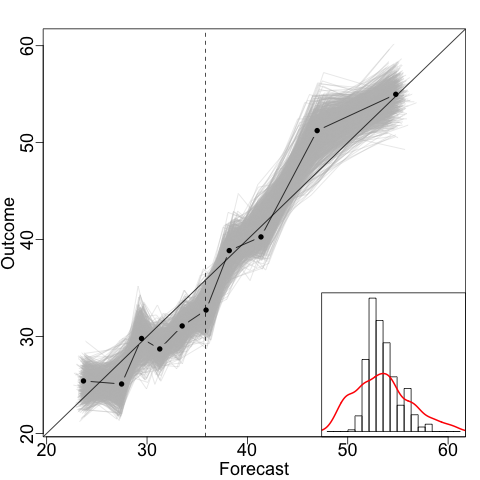
\includegraphics[width=\textwidth]{IndependentModel1}
                \caption{$\mathcal{M}_1$}
                \label{fig:gull}
        \end{subfigure}%
        ~ %add desired spacing between images, e. g. ~, \quad, \qquad, \hfill etc.
          %(or a blank line to force the subfigure onto a new line)
        \begin{subfigure}[b]{0.24\textwidth}
                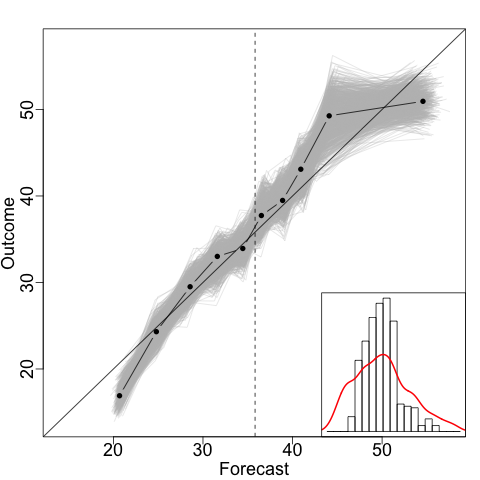
\includegraphics[width=\textwidth]{IndependentModel2}
                \caption{$\mathcal{M}_2$}
                \label{fig:tiger}
        \end{subfigure}
        \begin{subfigure}[b]{0.24\textwidth}
                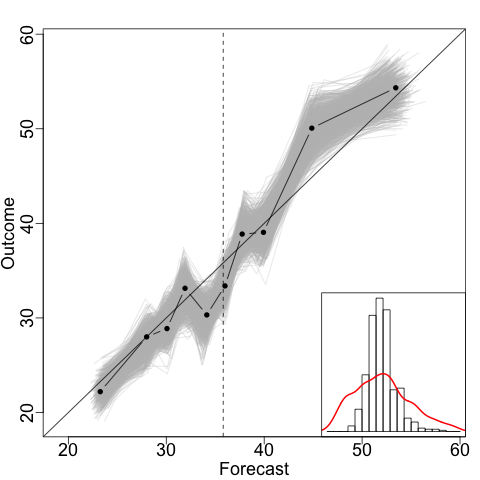
\includegraphics[width=\textwidth]{DependentModel2}
                \caption{$\mathcal{M}_3$}
                \label{fig:tiger}
        \end{subfigure}
                \begin{subfigure}[b]{0.24\textwidth}
                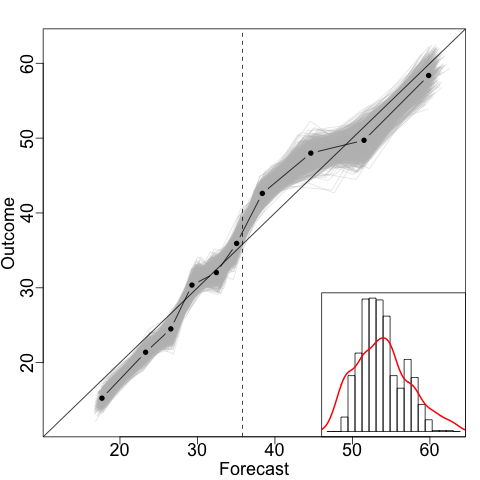
\includegraphics[width=\textwidth]{IndependentModelF}
                \caption{$\mathcal{M}_F$}
                \label{RelDiagramNoF}
        \end{subfigure}           
        \caption{Reliability diagrams of the models applied to the concrete compressive strength data.}
                
                \label{RelDiagramMo}
\end{figure}



\begin{figure}
        \centering
 
         %add desired spacing between images, e. g. ~, \quad, \qquad, \hfill etc.
          %(or a blank line to force the subfigure onto a new line)
        \begin{subfigure}[b]{0.323\textwidth}
                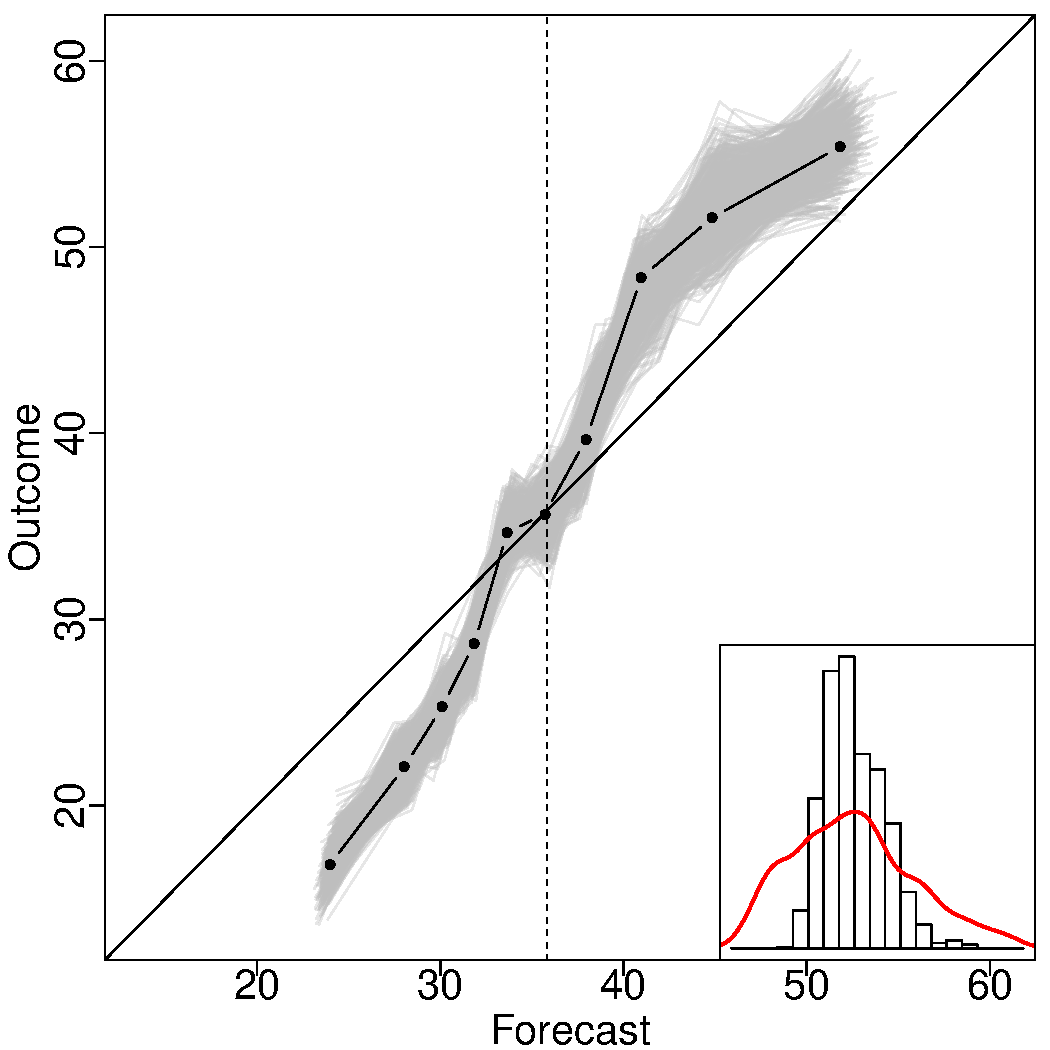
\includegraphics[width=\textwidth]{IndependentELP}
                \caption{$\bar{\mathcal{X}}$}
                \label{fig:mouse}
        \end{subfigure}
                  \begin{subfigure}[b]{0.323\textwidth}
                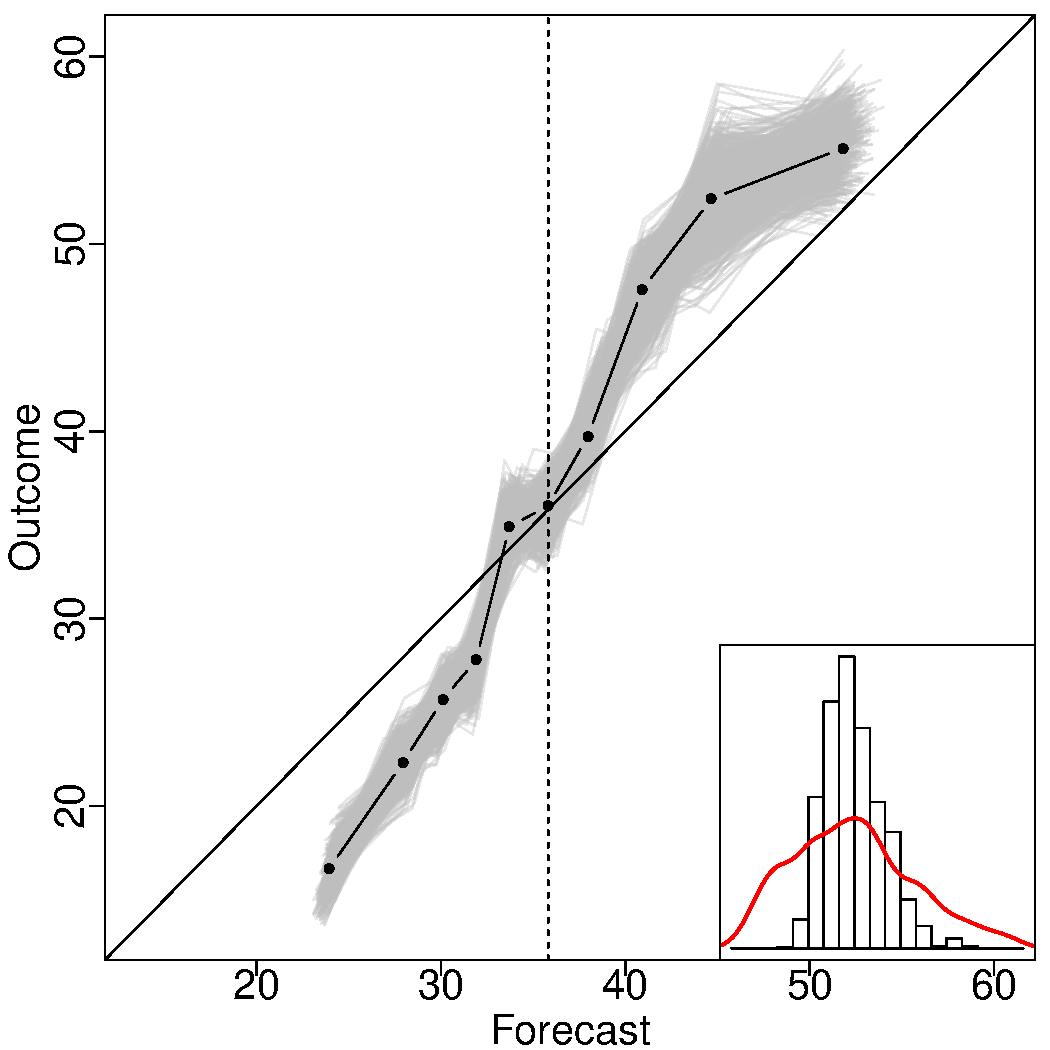
\includegraphics[width=\textwidth]{IndependentOLP}
                \caption{$\mathcal{X}_w$}
                \label{fig:gull}
        \end{subfigure}%
         \begin{subfigure}[b]{0.323\textwidth}
                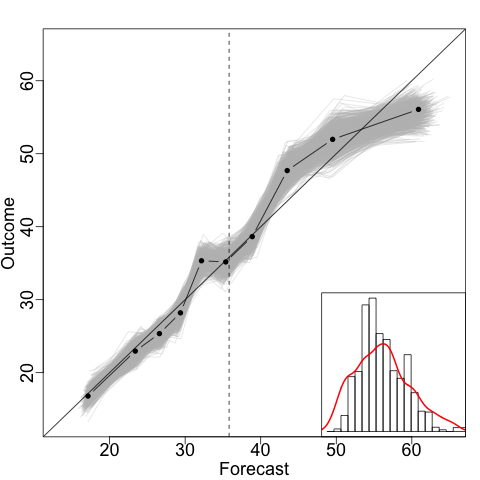
\includegraphics[width=\textwidth]{IndependentE-OLP}
                \caption{$\mathcal{X}^*$}
                \label{RelDiagramNoE}
             \end{subfigure}
        \caption{\textit{No Overlap.} Reliability diagrams of the competing aggregators under the concrete compressive strength data.}
                        \label{RelDiagramNo}
\end{figure}


\begin{figure}
        \centering
        \begin{subfigure}[b]{0.323\textwidth}
                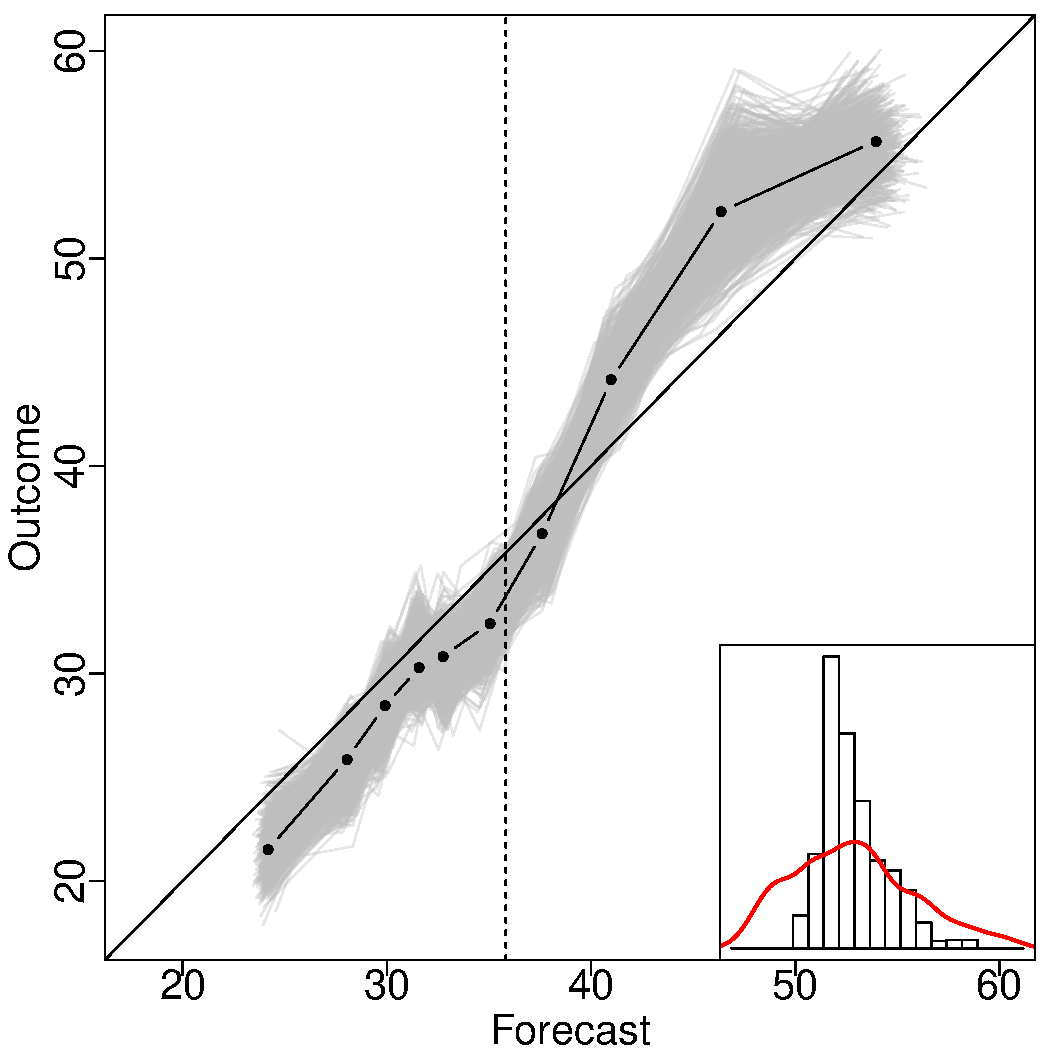
\includegraphics[width=\textwidth]{DependentELP}
                \caption{$\bar{\mathcal{X}}$}
                \label{fig:mouse}
        \end{subfigure}     
                \begin{subfigure}[b]{0.323\textwidth}
                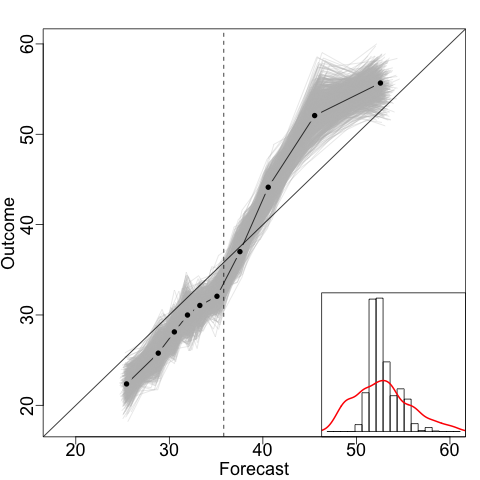
\includegraphics[width=\textwidth]{DependentOLP}
                \caption{$\mathcal{X}_w$}
                \label{fig:gull}
        \end{subfigure}%
        \begin{subfigure}[b]{0.323\textwidth}
                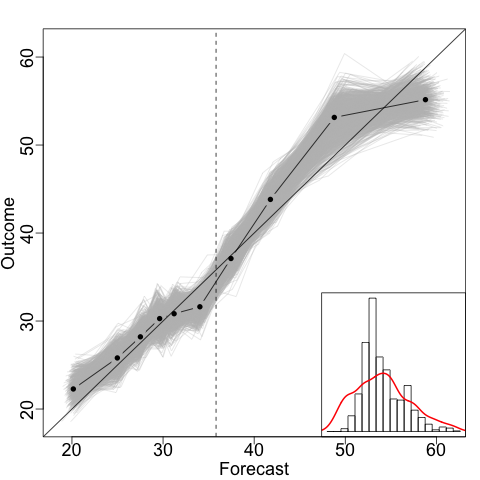
\includegraphics[width=\textwidth]{DependentE-OLP}
                \caption{$\mathcal{X}^*$}
                \label{DepEOLPConrete}
        \end{subfigure}
          \caption{\textit{High Overlap.}  Reliability diagrams of the competing aggregators under the concrete compressive strength data.}
               \label{RelDiagramHigh}
\end{figure}


Figures \ref{RelDiagramMo}, \ref{RelDiagramNo}, and \ref{RelDiagramHigh} presents the reliability diagrams of the individual models and the aggregators under both information scenarios. Unlike in Section \ref{simulation}, the marginal distribution of $Y$ is not known. Therefore the red curve over the inlined histogram represents the empirical distribution of $Y$. Similarly, the dashed vertical line represents the sample average of the outcomes instead of the marginal mean $\mu_0$. According to these plots, the individual forecasts are fairly reliable and do not present any systematic under- or over-confidence. Similarly to Section \ref{simulation}, the averaging aggregators $\bar{\mathcal{X}}$ and $\mathcal{X}_w$ are  unreliable and under-confident particularly in the no overlap scenario. Table \ref{NoParamsReal} shows the parameter estimates for $\mathcal{X}_w$ and $\mathcal{X}^*$. The weights employed by these two aggregators are very similar. However, in both information scenarios $\alpha > 1$, suggesting that $\mathcal{X}_w$ is under-confident and should be extremized as it is. Based on Figures \ref{RelDiagramNoE} and  \ref{DepEOLPConrete}, the resulting aggregator $\mathcal{X}^*$ is noticeably more reliable and appear to approximate the empirical distribution of $Y$ quite closely. Simply based on visual assessment $\mathcal{X}^*$ performs as well as $\mathcal{M}_F$ under low information overlap but  loses some resolution once  overlap is introduced. 

% latex table generated in R 3.2.0 by xtable 1.7-4 package
% Wed May 20 21:48:47 2015
\begin{table}[ht]
\centering
\caption{The estimated parameter values 
%of optimally weighted average, $\mathcal{X}_w$ and the extremized version of the optimally weighted average, $\mathcal{X}^*$ 
under the concrete compressive strength data. }
\begin{tabular}{llrrrr}
   \hline \hline
Scenario & Forecast & $\mu_0$ & $\alpha$ & $w_1$ & $w_2$\\
  \hline
\multirow{2}{*}{No Overlap} & $\mathcal{X}_w$ &  &  & 0.5327 & 0.4673 \\ 
&  $\mathcal{X}^*$ & -36.2051 & 1.6950 & 0.5269 & 0.4731 \\  \rule{0pt}{2.9ex} 
\multirow{2}{*}{High Overlap}  & $\mathcal{X}_w$ &  &  & 0.5931 & 0.4069 \\ 
 & $\mathcal{X}^*$ & -37.6776 & 1.4382 & 0.5375 & 0.4625 \\ 
   \hline
\end{tabular}
\label{NoParamsReal}
\end{table}

%\subsection{Concrete Compressive Strength}
% latex table generated in R 3.2.0 by xtable 1.7-4 package
% Fri May 15 16:06:28 2015
\begin{table}[h!]
\centering
\caption{The average quadratic loss, $L(\Y,\boldsymbol{\mathcal{X}} )$ with its three additive components: reliability (REL), resolution (RES), and uncertainty (UNC).The final column, $s(\boldsymbol{\mathcal{X}} )$ gives the estimated variance of the forecast. } 
\begin{tabular}{llrrrrr}
  \hline \hline
Scenario &  Forecast & $L(\Y,\boldsymbol{\mathcal{X}} )$ & REL & RES & UNC & $s(\boldsymbol{\mathcal{X}} )$\\ 
  \hline
 &  $\mathcal{M}_1$ & 187.80 & 9.70 & 100.72 & 278.81 & 82.83 \\ 
& $\mathcal{M}_2$  & 185.74 & 12.01 & 105.08 & 278.81 & 92.51 \\ 
  & $\mathcal{M}_3$ & 197.03 & 12.81 & 94.59 & 278.81 & 73.27 \\ 
&$\mathcal{M}_F$  & 110.91 & 9.46 & 177.36 & 278.81 & 157.87 \\ \rule{0pt}{2.9ex} 
\multirow{3}{*}{No Overlap} &  $\bar{\mathcal{X}}$ & 155.69 & 30.99 & 154.10 & 278.81 & 56.33 \\ 
 & $\mathcal{X}_w$ & 156.32 & 31.45 & 153.94 & 278.81 & 56.21 \\ 
  &$\mathcal{X}^*$ & 133.23 & 9.86 & 155.45 & 278.81 & 161.89 \\ \rule{0pt}{2.9ex} 
 \multirow{3}{*}{High Overlap}  & $\bar{\mathcal{X}}$ & 177.45 & 16.77 & 118.13 & 278.81 & 61.92 \\ 
  & $\mathcal{X}_w$ & 176.59 & 14.37 & 116.59 & 278.81 & 63.32 \\ 
 & $\mathcal{X}^*$ & 169.92 & 8.20 & 117.09 & 278.81 & 128.69 \\ 
\hline
\end{tabular}
\label{NoTbl}
\end{table}



Table \ref{NoTbl} provides a numerical comparison by presenting the average quadratic loss and its additive components under both information scenarios. Given that all aggregators perform better than the individual forecasters, aggregation is generally beneficial. However, there are large performance differences among the aggregators. In particular, the variances of $\bar{\mathcal{X}}$ and $\mathcal{X}_w$  do not exceed that of the individual forecasters', suggesting that neither of them is expanding. Furthermore, they are much less reliable than the individual forecasters. In contrast, $\mathcal{X}^*$ is able to maintain the forecasters' level of reliability. Even though it is expanding, it is less resolute and has a lower variance than $\mathcal{M}_F$. This can be expected because $\mathcal{X}^*$ has access only to a subset of the information that $\mathcal{M}_F$ uses. In the no overlap scenario, all the predictors are being used by the individual forecasters, but this does not mean that this information is actually revealed to $\mathcal{X}^*$ through the reported forecasts. 

\section{Conclusion and Future Research} \label{conclusion}

This paper discussed forecast aggregation under a general probability model, called the partial information framework. The forecasts and outcomes were assumed to have a joint distribution but no restrictions were placed on their dependence structure. This led to an enumeration (Theorem \ref{optimal}) of several properties of the optimal aggregator. Even though this aggregator is typically intractable in practice, its properties provide guidance for developing and understanding real-world aggregators. In this paper these properties shed light on the class of weighted averages of any type of univariate forecasts. Even though these averages are marginally consistent, they fail to satisfy two of the optimality properties, namely reliability and variance expansion (Theorem \ref{contraction}). As a results, they are under-confident in a sense that they are overly close to the marginal mean. This shortcoming can be alleviated by extremizing that shifts the weighted average further away from the marginal mean.  Section \ref{extremization} introduced a simple linear procedure (Equation \ref{firstProblem}) that extremizes the weighted average of real-valued forecasts and maintains marginal consistency while increasing variance. This procedure and the theoretical results were illustrated on synthetic (Section \ref{simulation}) and real-world data (Section \ref{application}). In both cases the optimally weighted average was shown to be both unreliable and under-confident, especially if the forecasters used very different sets of information. Fortunately, extremization largely corrected these drawbacks and provided transformed aggregates that were both reliable and highly resolute. 

Forecast aggregation literature by and large agrees that the goal is to collect and combine  information from different forecasters (see, e.g., \citealt{forlines2012heuristics, armstrong2, dawid1995coherent}). At the same time aggregation continues to be performed via weighted averaging or perhaps some other measure of central tendency, such as the median \citep{armstrong2, levins1966strategy, lobo2010human}. Section \ref{contraction} explained that these popular techniques do not behave like aggregators of information. They are designed to reduce measurement error which is philosophically very different from information diversity \citep{satopaamodeling2}. Therefore some details of their workings have been generally misunderstood.
% do not operate in the manner that they are believed to operate. 
% some of the workings of these techniques have been misunderstood or the role of the techniques is . Therefore, 

This paper illustrated that information aggregation can arise from very simple extremization techniques. However, learning the amount and direction of extremization requires a training set with known outcomes. Such a training set may not always be available. In the most extreme case  the decision-maker may have only a set of forecasts of a single unknown outcome. How should the forecasts be aggregated in such a low-data setting? The results in this paper suggest that any type of weighted average (or some other measure of central tendency) is a poor choice. A better alternative was discussed by \cite{satopaamodeling}. They assume that the forecasters' covariance matrix is compound symmetric and then aggregate the forecasts with the optimal aggregator under the corresponding Gaussian partial information model. 
%Intuitively, this aggregator assumes that the forecasters sample information sources from a common distribution. 
%requires an assumption on the structure of the covariance matrix of the forecasts. 
% In general, it is not clear what aggregator should be used.
 Developing other aggregators that place less constraints on the joint dependence structure while satisfying at least two of the optimality properties of Theorem \ref{optimal} is certainly an interesting future research direction. The first step is to develop an aggregator that is both marginally consistent and expanding. Finding an aggregator that maintains forecasters' reliability seems more difficult. 
% Meanwhile, the analysis of the general revealed aggregator should continue to explore other optimality properties.

%\marginpar{Time to find new class of inflation aggregators; the averages just do not do this.}
%\marginpar{Be more explicit about what we want to find: aggregator with no tuning parameters. Can integrate our.}

%  with the hope of finding more optimality properties.
%  should be explored by further analyzing the revealed aggregator. 


%
%
%This paper makes the first step by pointing out the mismatch. The next step is to convince the practitioners by developing a set of aggregators to replace the measurement-error based aggregators. This in particular involves a continued exploration of the properties of the optimal revealed aggregator. 
%
%
%This paper makes the first points out the mismatch between 
%
%
%It is clear that this misunderstanding must be  corrected and the methodological gap closed by 
%
%The first step  it is clear that forecast aggregation must move away from the measurement-error based aggregators and 
%
%
%
%
%Levins (1966), a biologist, suggested that rather than building one master
%model, it is often better to build several simple models that, among them, use all the information available and then
%average them. I

\appendix
\section{Appendix}
\subsection{Proof of Theorem \ref{optimal}}
%\begin{proof}
\begin{enumerate}[i)]
\item The law of total expectation gives:
\begin{align*}
\E(\mathcal{X}'') &= \E[\E(Y|\mathcal{X}'')] =  \E(Y) = \mu_0.
\end{align*}

\item Recall that $ \mathcal{X}'' = \E(Y | \F'')$ and $\mathcal{X}'' \in \F''$. Then,
\begin{align*}
\E(Y | \mathcal{X}'') &= \E[\E(Y|\mathcal{X}'',\F'')|\mathcal{X}'']\\
&= \E[\E(Y|\F'')|\mathcal{X}'']\\
&= \E(\mathcal{X}''|\mathcal{X}'') \\
&= \mathcal{X}''.
\end{align*}

\item This relies on the observation that $\sigma(X_j) = \F_j \subseteq \F'' = \sigma(X_1, \dots, X_N)$. Then,
\begin{align*}
\delta_{max} &=\Var(\mathcal{X}'')\\
 &= \E\left(X_j^2\right) - \mu_0^2\\
 &= \E[\E(Y|\F_j)X_j] - \mu_0^2\\
 &= \E\{\E[\E(Y|\F'')|\F_j]X_j\} - \mu_0^2 & \text{(the smallest $\sigma$-field wins)}\\
 &= \E[\E(\mathcal{X}''|\F_j)X_j] - \mu_0^2 \\
 &= \E(\mathcal{X}''X_j) - \mu_0^2 \\
 &= \E[(\mathcal{X}''-\mu_0)(X_j-\mu_0)]  \\
 &\leq \sqrt{\Var(\mathcal{X}'')\delta_{max} } & \text{(by the Cauchy-Schwarz inequality)} 
\end{align*}
Squaring and diving both sides by $\delta_{max} $ gives the desired result. 

\end{enumerate}
%\end{proof}
\qed

\subsection{Proof of Theorem \ref{contraction}}
%\begin{proof}
Items ii) and iii) are generalizations of the proof in \cite{Ranjan08}. 
\begin{enumerate}[i)]
\item
% Given that $X_j$ for all $j = 1, \dots, N$ are integrable,
%\begin{align*}
%\E(|\w'\X|) &\leq \sum_{j=1}^N \E(|w_jX_j|) & \text{ (by the triangle inequality)}\\
%&= \sum_{j=1}^N w_j \E(|X_j|)\\
%&< \infty
%\end{align*}
This follows from direct computation:
\begin{align*}
\E(\mathcal{X}_w) = \E(\w' \X) &= \w' \E(\X) = \mu_0 \w' \one_N = \mu_0.
\end{align*}

%This follows from direct computation:
%\begin{align*}
%\E[X''] &= \E[\E[Y|X'']] = \mu_0\\
%\end{align*}
\item Consider some reliable aggregate $\mathcal{X}$ such that $\E(Y | \mathcal{X}) = \mathcal{X}$. Then,
\begin{align*}
\E[(Y-\mathcal{X})^2] &= \E\left\{\E\left[(Y-\mathcal{X})^2|\mathcal{X}\right]\right\}\\
&= \E\left[\E\left(Y^2-2Y\mathcal{X}+\mathcal{X}^2|\mathcal{X} \right)\right]\\
&= \E\left[\E\left(Y^2|\mathcal{X}\right)-\mathcal{X}^2\right]\\
&= \E(Y^2)-\E(\mathcal{X}^2)
\end{align*}
The rest of the proof shows that if $\mathcal{X} = \mathcal{X}_w = \w'\X$, then the above identity cannot hold. This gives a contradiction and hence proves the desired result. First, note that $\sum_{i=1}^N\sum_{j=1}^Nw_iw_j = 1$. Then,
\begin{align*}
\E\left[\left(Y-\mathcal{X}_w\right)^2\right] &= \E\left[\left(Y-\w'\X\right)^2\right] \\
 &= \E\left\{\left[\sum_{j=1}^Nw_j (Y-X_j)\right]^2\right\} \\
% &= \E[Y^2-2Y\w'\X+\w'\X\X'\w] \\
% &= \E[\sum_{i=1}^N\sum_{j=1}^N w_iw_j Y^2-2Y\w'\X+\sum_{i=1}^N\sum_{j=1}^N w_iw_j X_iX_j] \\
&= \sum_{i=1}^N\sum_{j=1}^Nw_iw_j \E[(Y-X_i)(Y-X_j)] \\
&= \sum_{i=1}^N\sum_{j=1}^Nw_iw_j \E\left(Y^2-YX_i-YX_j+X_jX_i\right) \\
&= \sum_{i=1}^N\sum_{j=1}^Nw_iw_j \E\left[ \E\left( Y^2|X_i \right)-\E\left( YX_i|X_i \right)-\E\left( YX_j|X_j\right)+X_jX_i \right] \\
&= \sum_{i=1}^N\sum_{j=1}^Nw_iw_j \E\left[ \E\left( Y^2|X_i \right)-X_i^2-X_j^2+X_jX_i \right] \\
&= \sum_{i=1}^N\sum_{j=1}^Nw_iw_j \E\left[\E\left(Y^2|X_i\right) +\left(X_jX_i-X_jX_i\right)-X_i^2-X_j^2+X_jX_i\right] \\
&= \sum_{i=1}^N\sum_{j=1}^Nw_iw_j \E\left[\E\left(Y^2|X_i\right) -X_jX_i-\left(X_i-X_j\right)^2\right] \\
&= \sum_{i=1}^N\sum_{j=1}^Nw_iw_j \E\left[\E\left(Y^2|X_i\right) -X_jX_i\right]-\sum_{i=1}^N\sum_{j=1}^Nw_iw_j\E\left[\left(X_i-X_j\right)^2\right] \\
&=  \E\left(Y^2\right) - \sum_{i=1}^N\sum_{j=1}^Nw_iw_j \E\left(X_jX_i\right)-\sum_{i=1}^N\sum_{j=1}^Nw_iw_j\E\left[\left(X_i-X_j\right)^2\right] \\
&=  \E\left(Y^2\right) -  \E\left(\w'\X \X'\w\right)-\sum_{i=1}^N\sum_{j=1}^Nw_iw_j\E\left[\left(X_i-X_j\right)^2\right] \\
&= \left[\E\left(Y^2\right) -  \E\left(\mathcal{X}_w\right) \right]-\sum_{i=1}^N\sum_{j=1}^Nw_iw_j\E\left[\left(X_i-X_j\right)^2\right].
\end{align*}
This leads to a contraction because the double sum on the final line is strictly positive as long as there exists a pair $i \neq j$ such that $\P(X_i \neq X_j) > 0$ and $w_i, w_j > 0$. 

\item The fact that $\E(\mathcal{X}_w') = \mu_0$ follows from the same steps as shown in item i) of Theorem \ref{optimal}. Then,
\begin{align*}
\E \left[ \left( Y - \mathcal{X}_w\right)^2\right] &= \E \left( Y^2 - 2Y\mathcal{X}_w + \mathcal{X}_w^2\right)\\
&= \E \left( Y^2 + 2\left(\mathcal{X}_w'^2-\mathcal{X}_w'^2\right)- 2Y\mathcal{X}_w + \mathcal{X}_w^2\right)\\
&= \E \left( Y^2 -2Y\mathcal{X}_w'+2\mathcal{X}_w'^2- 2\mathcal{X}_w'\mathcal{X}_w + \mathcal{X}_w^2\right)\\
&= \E\left[\left(Y-\mathcal{X}_w'\right)^2\right] + \E\left[\left(\mathcal{X}_w-\mathcal{X}_w'\right)^2\right] \\
&= \E(Y^2)-\E(\mathcal{X}_w'^2) + \E\left[\left(\mathcal{X}_w-\mathcal{X}_w'\right)^2\right] & \text{(because $\mathcal{X}_w'$ is reliable)}\\
&> \E(Y^2)-\E(\mathcal{X}_w'^2) 
\end{align*}
Furthermore, from the previous item, $\E \left[ \left( Y - \mathcal{X}_w\right)^2\right] < \E(Y^2)-\E(\mathcal{X}_w^2)$. Putting this all together gives
\begin{align*}
&&\E(Y^2)-\E(\mathcal{X}_w'^2)  &< \E(Y^2)-\E(\mathcal{X}_w^2)\\
%\E(\mathcal{X}_w'^2)  &> \E(\mathcal{X}_w^2)\\
\Leftrightarrow && \E(\mathcal{X}_w'^2) - \mu_0^2  &> \E(\mathcal{X}_w^2) - \mu_0^2\\
\Leftrightarrow && \Var(\mathcal{X}_w')  &> \Var(\mathcal{X}_w^2)
\end{align*}


%Given that $\mathcal{X}_w'$ is reliable, the previous item gives $\E\left[\left(Y-\mathcal{X}_w'\right)^2\right] =\E(Y^2)-\E(\mathcal{X}_w'^2)$. 

\item The fact that $\Var(\mathcal{X}_w)\leq \delta_{max}$ follows from direct computation:
\begin{align*}
\Var(\mathcal{X}_w) &= \E[(\mu_0 - \mathcal{X}_w)^2]\\
% &= \E(\mu_0^2 - 2\mu_0\mathcal{X}_w + \mathcal{X}_w^2)\\
&= \E(\mathcal{X}_w^2) - \mu_0^2\\
&= \w' \E(\X \X')\w - \w'\one_N \mu_0^2\one_N'\w\\
&= \w' \left[ \E(\X \X') - \mu_0^2 \one_N \one_N' \right]\w\\
&= \w' \E[(\X - \one_N \mu_0)(\X - \one_N \mu_0)']\w\\
&= \w' \Cov(\X)\w\\
&\leq \delta_{max} \one_N'\w\\
&= \delta_{max}.
\end{align*}

To see the identity part of the statement, note that $$\Var(\mathcal{X}_w)  = \w' \Cov(\X)\w = \Sigma_{i=1}^N \Sigma_{k=1}^N w_{ik} \Cov(X_i, X_k),$$ where $w_{ik} = w_iw_k \in [0,1]$ and $\sum_{i=1}^N \sum_{k=1}^N w_{ik} = 1$.  First, suppose that $\Var(X_j) = \delta_{max} > \Var(X_i) = \delta_i$ for all $i \neq j$. Then, if $w_{ii} > 0$ for some $i \neq j$, the term $w_{ii}\Cov(X_i, X_i)$ brings $\Var(\mathcal{X}_w)$ below $\delta_{max}$. This decrease cannot be compensated by any other term because no element in $\Cov(\X)$ is larger than $\delta_{max}$. Consequently, it must be case that $w_i = 0$ for all $i \neq j$. Now, if there exists $k \neq j$ such that $\delta_k = \delta_{max}$ and $w_k > 0$, then $\Var(\mathcal{X}_w) = \delta_{max}$ only if all weight is given to $X_j$ and $X_k$, and $\Cov(X_k, X_j) = \delta_{max}$. This covariance implies that $\Corr(X_k, X_j) = 1$. Thus, $\sigma(X_k) = \sigma(X_j)$ and hence that $X_k = \E[Y | \sigma(X_k)] = \E[Y | \sigma(X_j)] = X_j$. Consequently, $\Var(\mathcal{X}_w) = \delta_{max}$ only if all weight is distributed among $X_i$ such that $X_i = X_j$. 

 From the Theorem \ref{optimal}, $\delta_{max} \leq \Var(\mathcal{X}'')$, where the inequality arises from the Cauchy-Schwarz inequality. It is well-known that this reduces to an equality if and only if $\mathcal{X}''$ and $X_j$ are linearly dependent. Such a linear dependence would imply that $\sigma(\mathcal{X}'') = \sigma(X_j)$ and hence that $X_j = \E[Y | \sigma(X_j)] = \E[Y | \sigma(\mathcal{X}'')] = \mathcal{X}''$. Now, if there exists $k \neq j$ such that $\delta_k = \delta_{max}$, then by the same argument $\sigma(\mathcal{X}'') = \sigma(X_j) = \sigma(X_k)$ and consequently $X_k = X_j = \mathcal{X}''$. 

Putting this all together gives that $\w'\X = \mathcal{X}''$ if and only if $\sigma(X_j) = \sigma(\mathcal{X}'')$ and $w_i > 0$ only for all $X_i = X_j$.

\end{enumerate}
%\end{proof}
\qed

\subsection{Derivation of Equation \ref{decomposition}}
Suppose that $\mathcal{X}_k \in \{f_1, \dots, f_I\}$ for some finite $I$. Then,
\begin{align*}
& \frac{1}{K} \sum_{k=1}^K (Y_k - \mathcal{X}_k)^2\\
 &= \frac{1}{K} \left( \sum_{k=1}^K \mathcal{X}_k^2 - 2\sum_{k=1}^KY_k\mathcal{X}_k + \sum_{k=1}^KY_k^2 \right)\\
 &= \frac{1}{K} \left[ \sum_{i=1}^I K_i f_i^2 - 2\sum_{i=1}^I K_i f_i \bar{Y}_i + \left( 2 \sum_{i=1}^IK_i\bar{Y}_i\bar{Y}- 2 \sum_{i=1}^IK_i\bar{Y}_i\bar{Y} \right) +  \left( \sum_{i=1}^IK_i\bar{Y}^2- \sum_{i=1}^IK_i\bar{Y}^2 \right) + \sum_{k=1}^KY_k^2 \right]\\
 &= \frac{1}{K} \left[ \sum_{i=1}^I K_i \left( f_i^2 - 2 f_i \bar{Y}_i + 2 \bar{Y}_i\bar{Y}-  \bar{Y}^2 \right) + \sum_{k=1}^K(Y_k^2 -2\bar{Y}_k\bar{Y}+ \bar{Y}^2) \right]\\
 &= \frac{1}{K} \left[ \sum_{i=1}^I K_i \left( f_i^2 - 2 f_i \bar{Y}_i + (\bar{Y}_i^2 - \bar{Y}_i^2) + 2 \bar{Y}_i\bar{Y}-  \bar{Y}^2 \right) + \sum_{k=1}^K(Y_k -\bar{Y})^2 \right]\\
 &= \frac{1}{K} \left[ \sum_{i=1}^I K_i \left( f_i^2 - 2 f_i \bar{Y}_i + \bar{Y}_i^2 \right)  - \sum_{i=1}^I K_i  \left(\bar{Y}_i^2 - 2 \bar{Y}_i\bar{Y} + \bar{Y}^2 \right) + \sum_{k=1}^K(Y_k -\bar{Y})^2 \right]\\
 &=  \frac{1}{K} \sum_{i=1}^I K_i \left( f_i - \bar{Y}_i \right)^2  - \frac{1}{K} \sum_{i=1}^I K_i  \left(\bar{Y}_i - \bar{Y} \right)^2 + \frac{1}{K} \sum_{k=1}^K(Y_k -\bar{Y})^2.
\end{align*}





%\bibliographystyle{plain}
\bibliographystyle{apalike}
\bibliography{biblio}		% expects file "myrefs.bib"

\end{document}
